Cette section cherche à caractériser la nature des solutions du problème d’isopérimétrie polygonale.
Compte-tenu du fait \ref{at-least-one-ncycle}, nous pourrions raisonner avec des \ncycles\ convexes,%
\footnote{
	Par exemple, pour justifier qu'un \ngone\ non convexe $\setproba{P}$ n'est pas optimal, il suffit d'exhiber un \ncycle\ convexe $\setproba{L}$ qui vérifie
$\cyclelen{\setproba{L}} = \cyclelen{\setproba{P}}$,
	ainsi que
	$\area{\setproba{L}} > \area{\setproba{P}}$.
}
mais nous allons tout de même nous restreindre aux \ngones, car cela ne demande que peu d'efforts supplémentaires, tout en fournissant de jolis résultats.

\begin{tcolorbox}
	\itshape\small
	Comme les cas $n = 3$ et $n = 4$ ont été résolus, voir les faits \ref{iso-tri} et \ref{quadri}, pour ne pas alourdir le texte, nous supposerons $n \geq 5$ dans toutes les preuves de cette section.
\end{tcolorbox}


% ----------------------- %


Commençons par un fait simple, mais utile, qui mérite d'être mis en valeur.


\begin{fact} \label{bigger-convex}
    Si $\setproba{P}$ est un \ngone\ convexe, $s \in \NNs$ et $L \in \RR_{>\cyclelen{\setproba{P}}}$,
    alors il existe un \xgone{(n+s)}\ convexe $\setproba{C}$ tel que
	$\cyclelen{\setproba{P}} < \cyclelen{\setproba{C}} < L$
	et
	$\area{\setproba{P}} < \area{\setproba{C}}$.
\end{fact}


\begin{proof}
    Intuitivement, il suffit d'ajouter des points suffisamment proches d'un côté, et à l'extérieur, comme l'illustre la figure suivante.
    %
    \begin{center}
        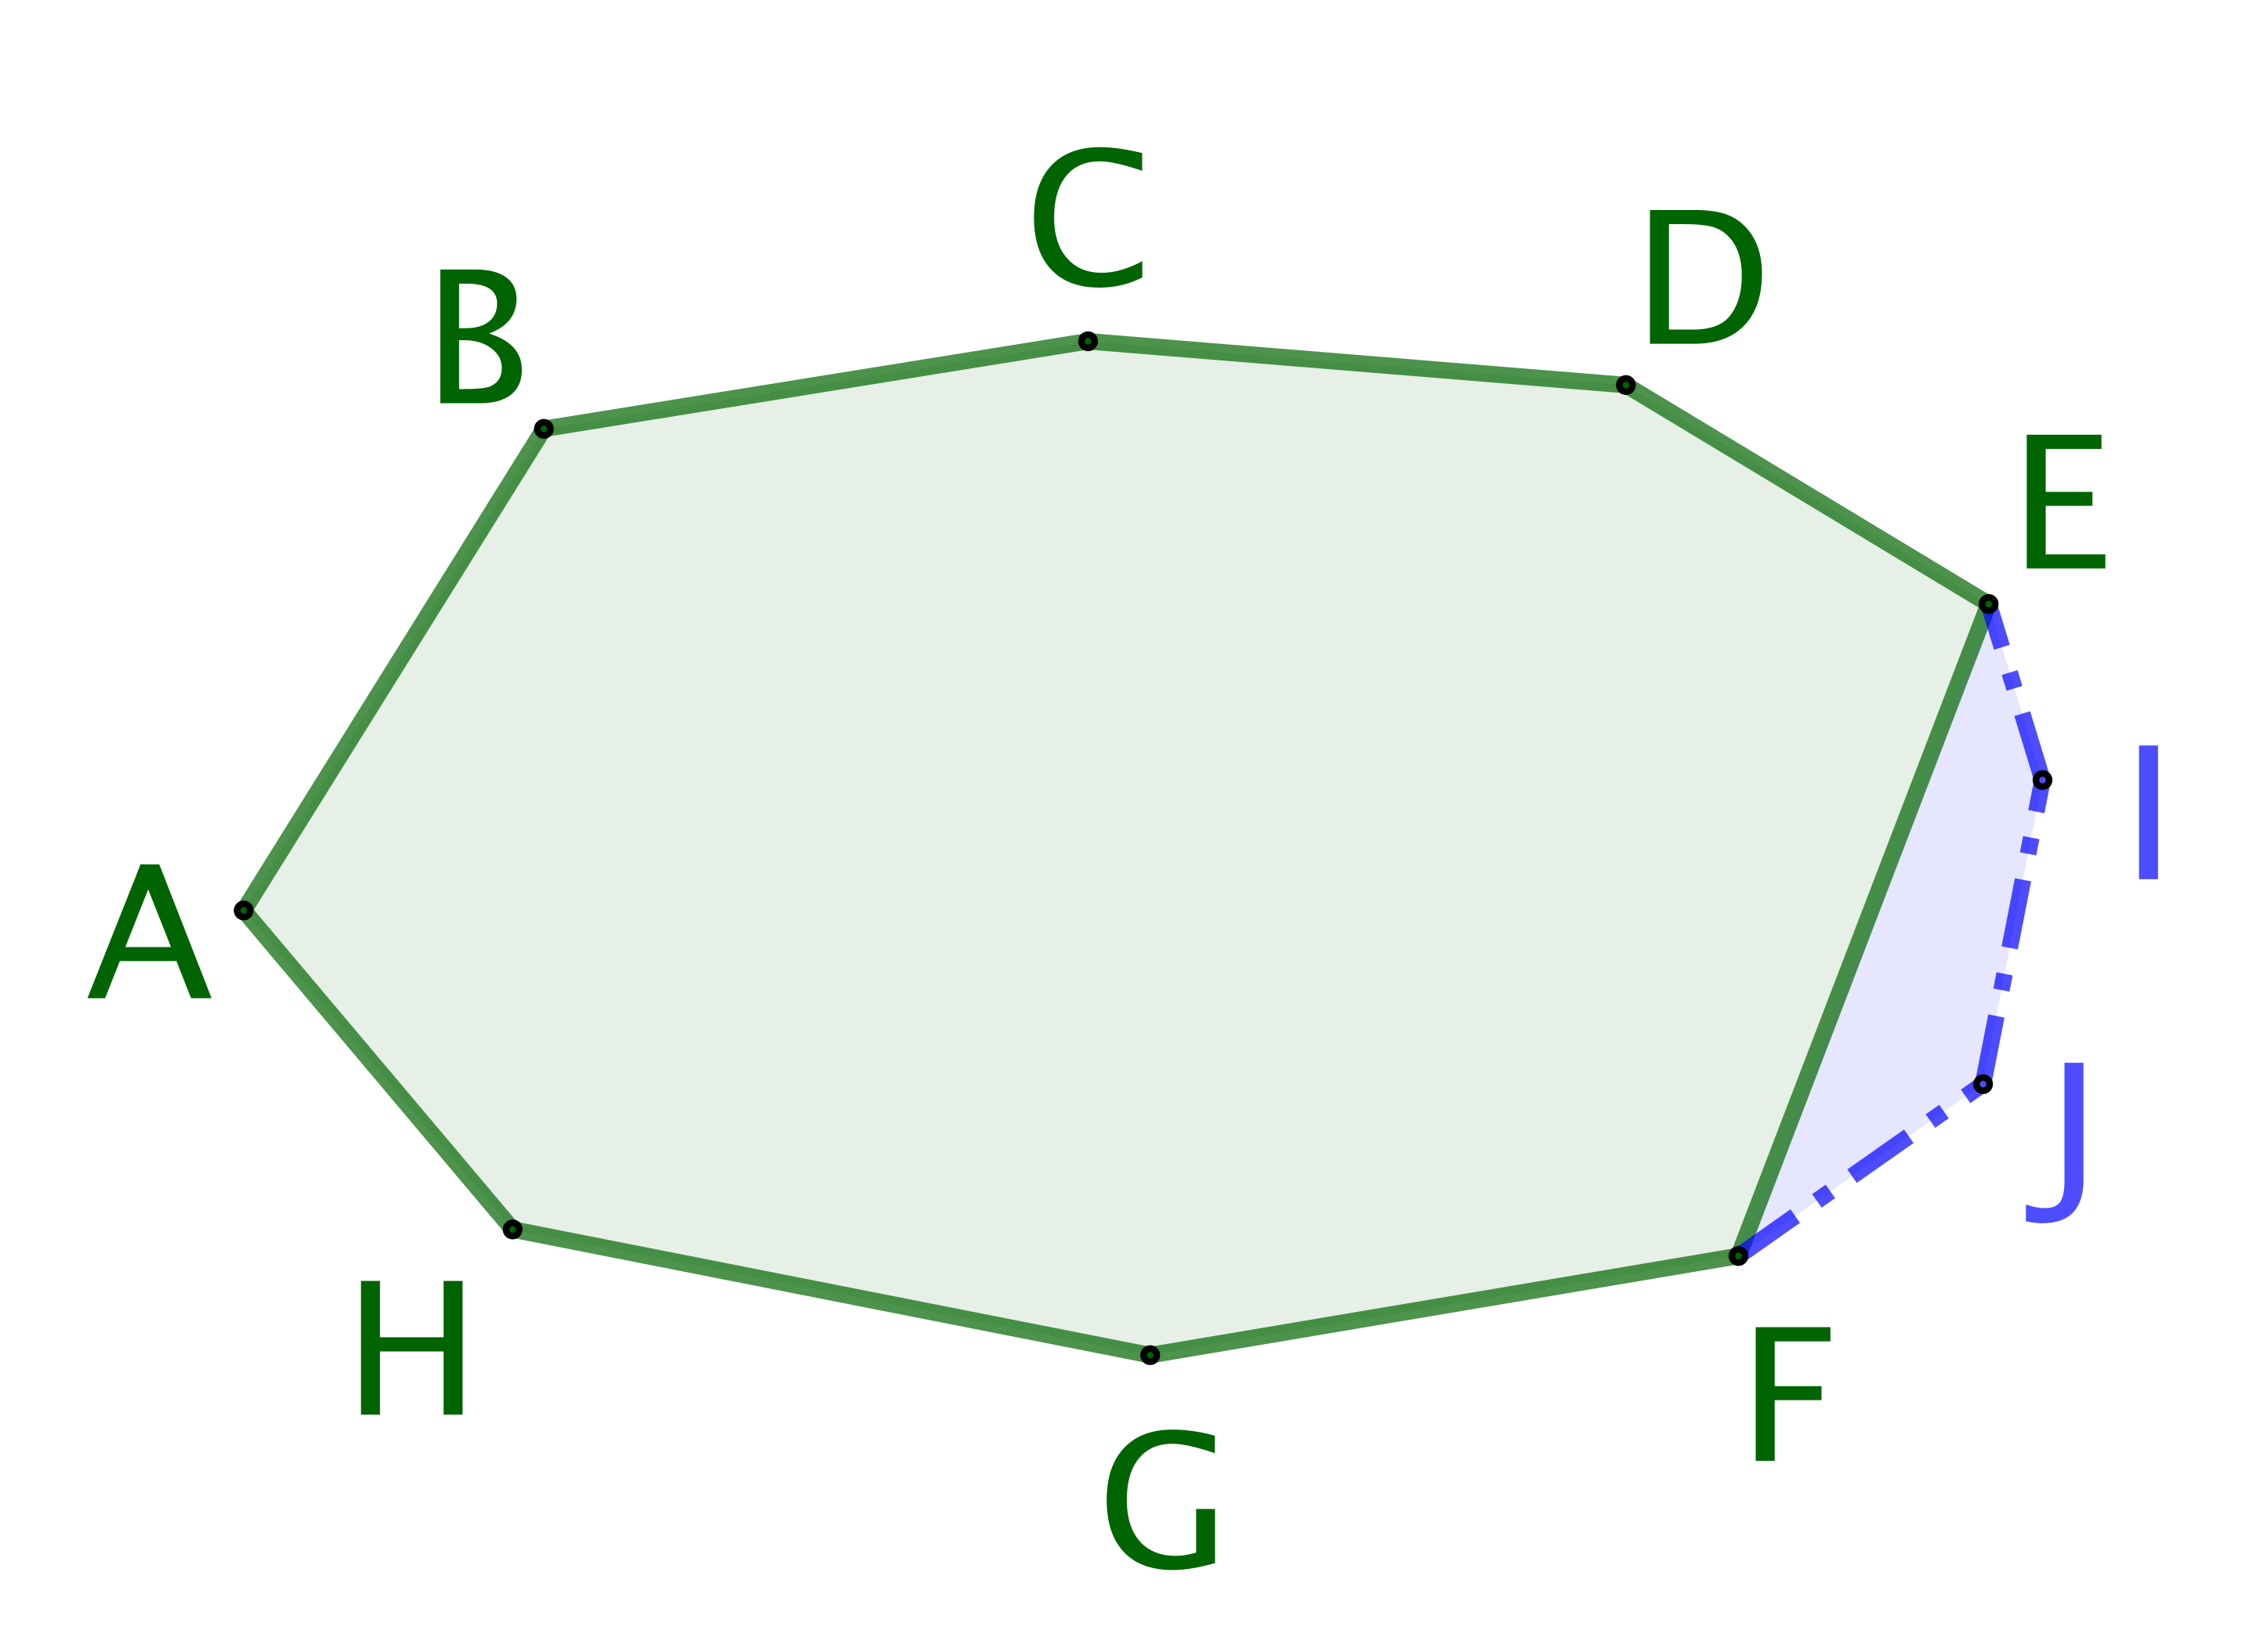
\includegraphics[scale=.4]{bigger-convex.png}
    \end{center}
    
    Pour formaliser proprement notre idée, posons
	$\delta = \frac{L - \cyclelen{\setproba{P}}}{s}$ qui est tel que $\delta > 0$.
	%
	\begin{enumerate}
		\item \label{add-vertex-start}
		Considérons $[AB]$ un côté quelconque de $\setproba{P}$.
		Les droites portées par les côtés contigus à $[AB]$ \focus{dessinent} une région hachurée contenant toujours un triangle $ABC$ dont l'intérieur est à l'extérieur
		\footnote{
			C'est ce que l'on appelle de la \focus{low poetry}.
		}
		de $\setproba{P}$ comme dans les deux cas ci-dessous.
		%
		\begin{multicols}{2}
			\centering

			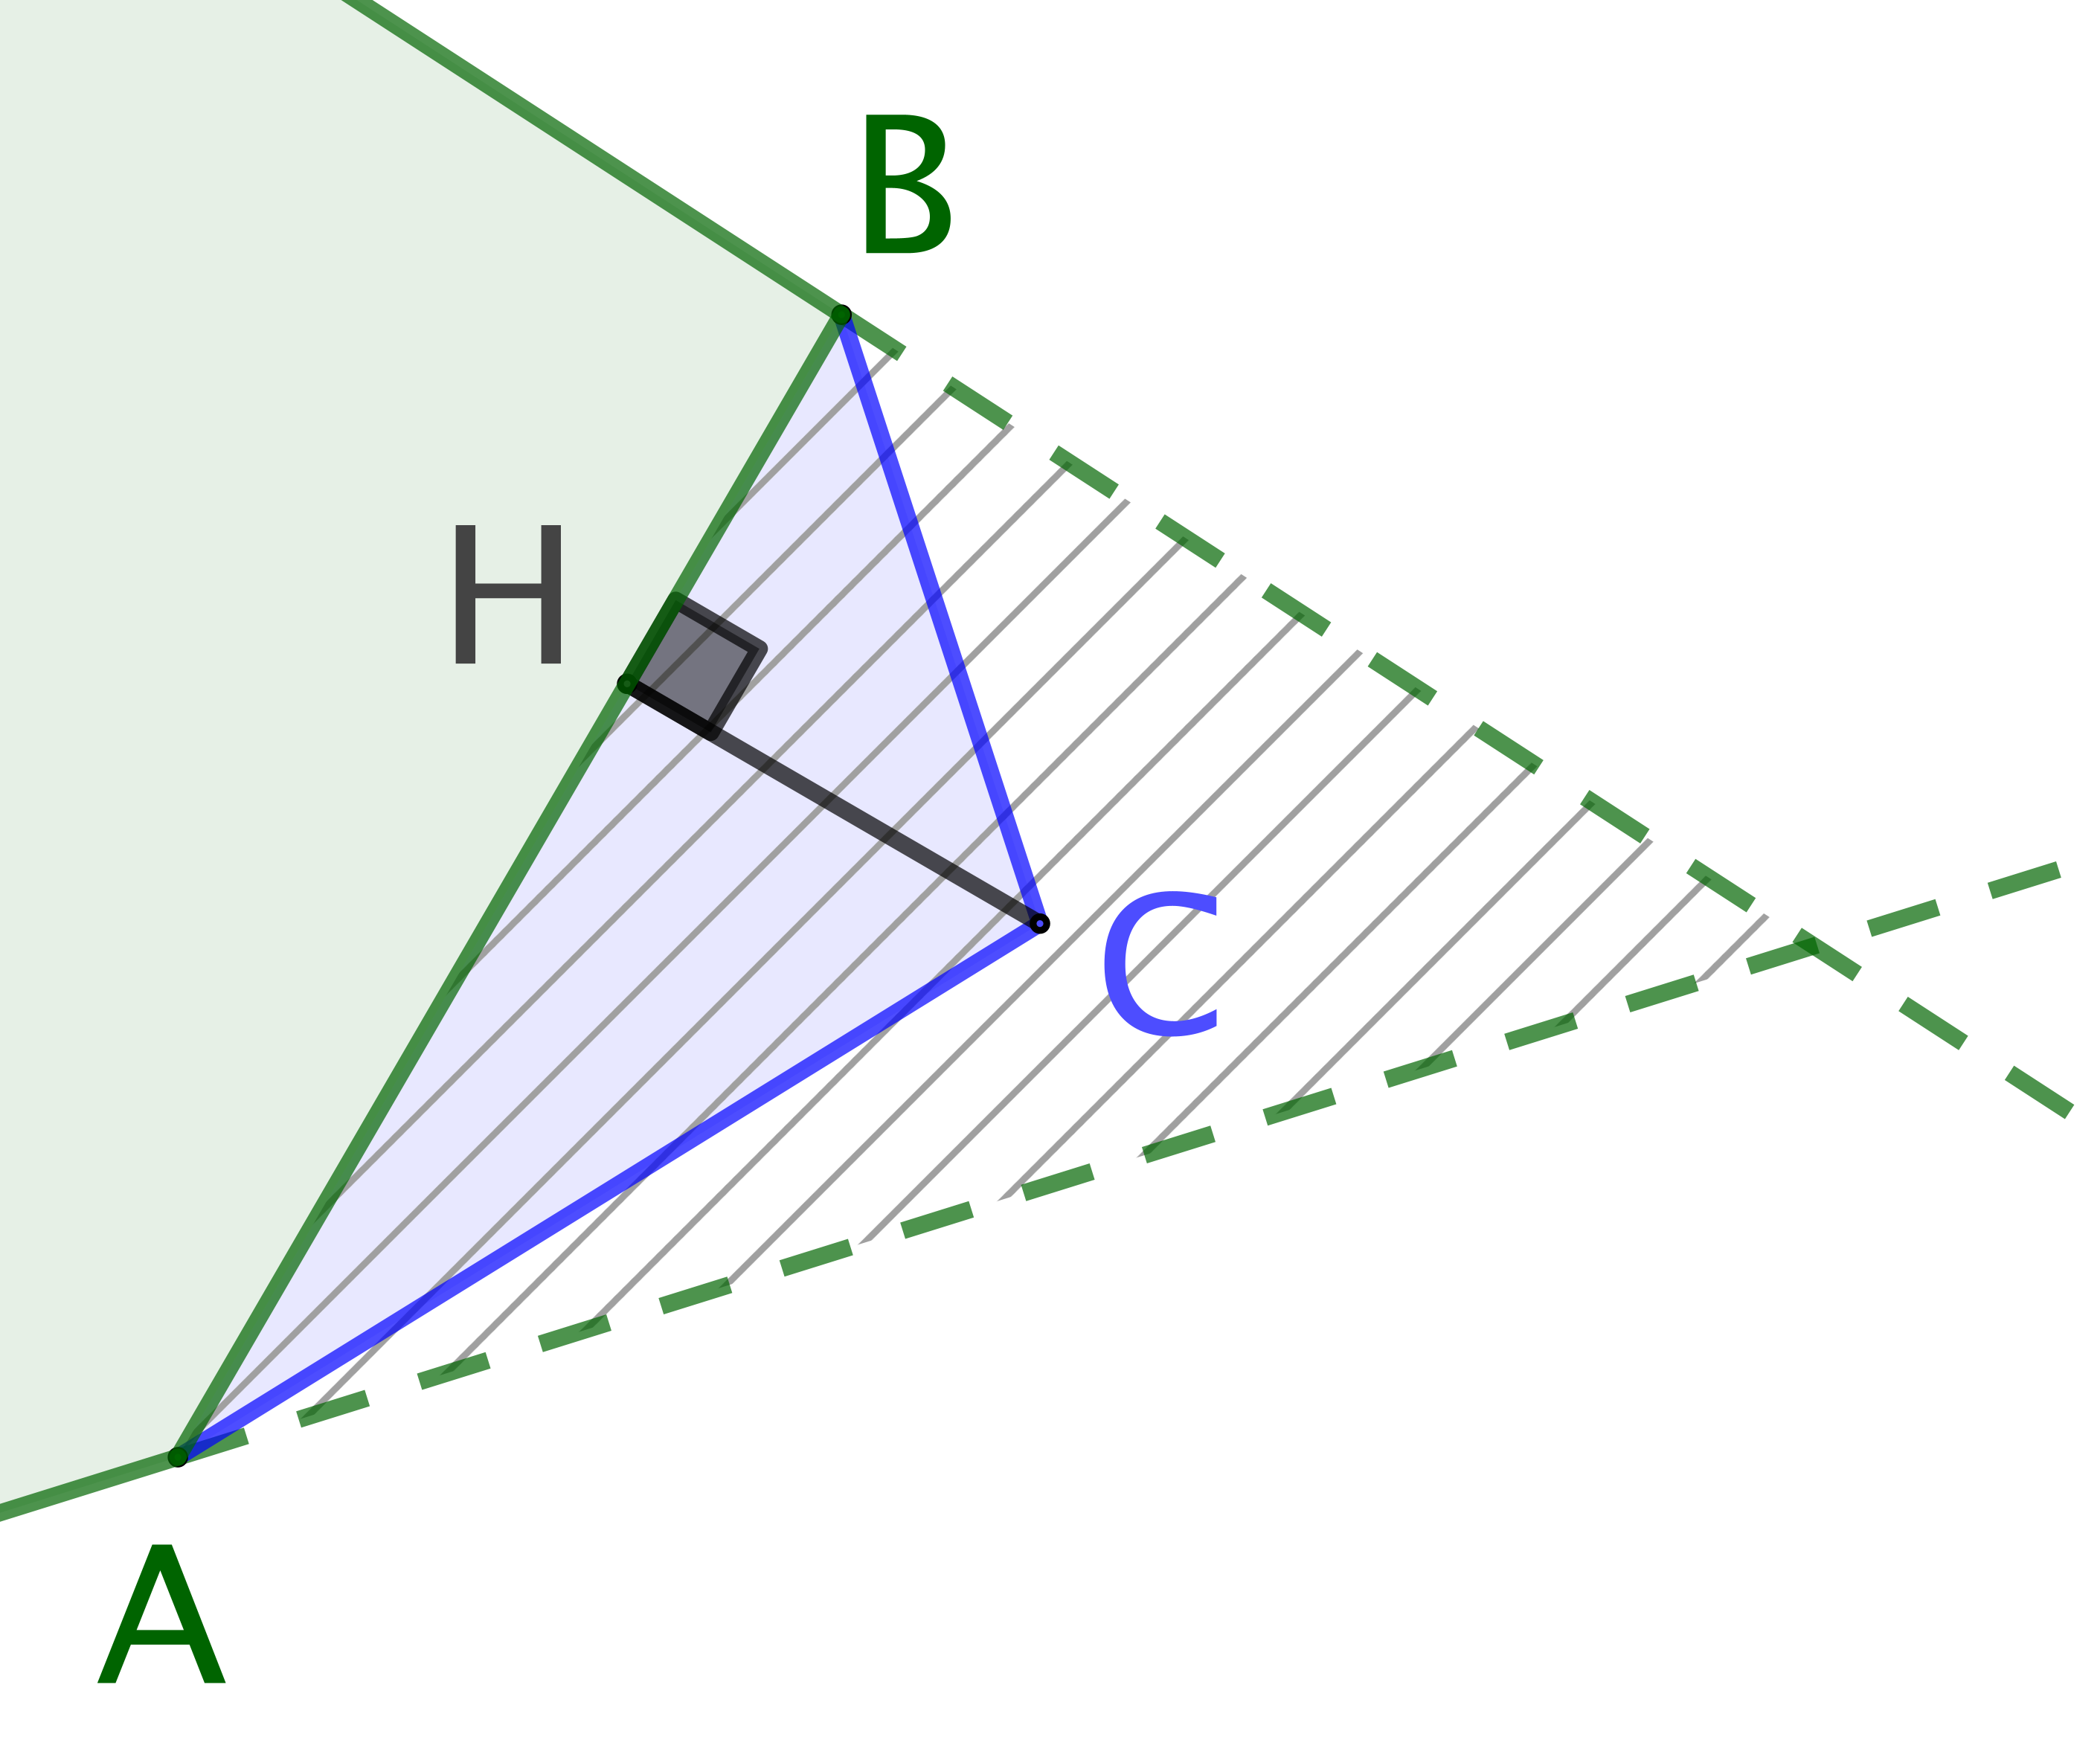
\includegraphics[scale=.35]{content/polygon/sol-must-be/add-vertex-1.png}

			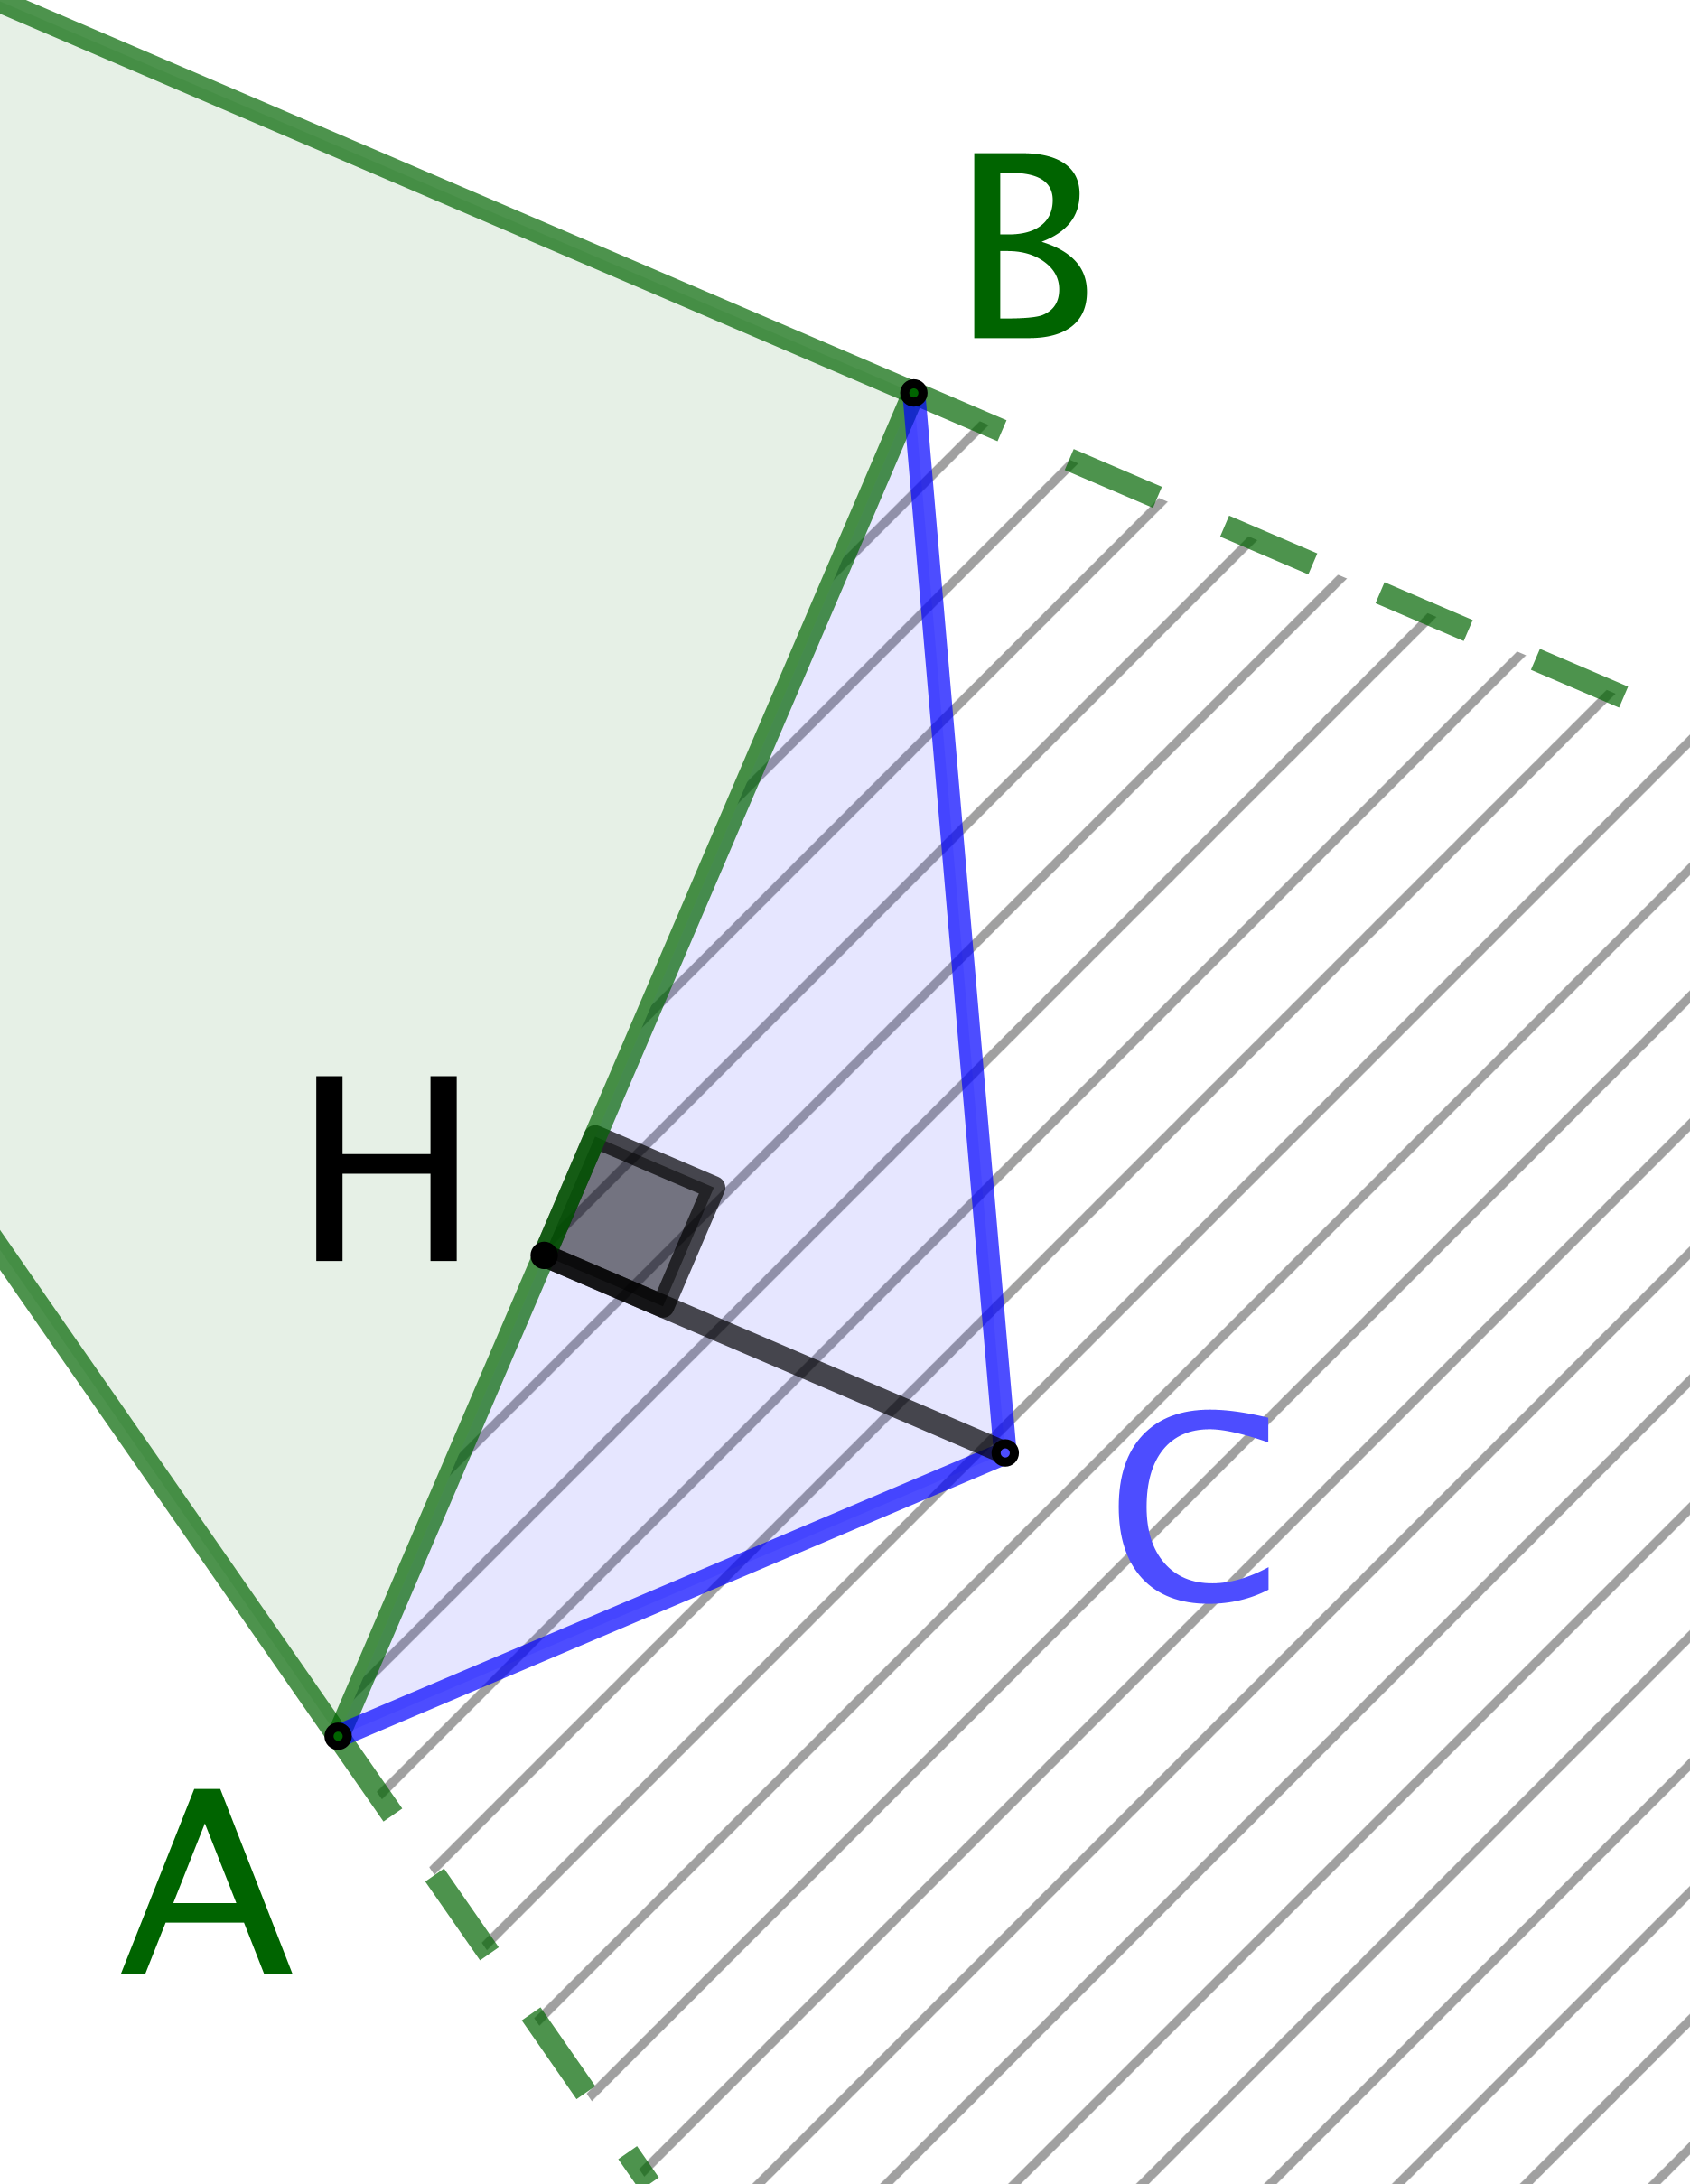
\includegraphics[scale=.3]{content/polygon/sol-must-be/add-vertex-2.png}
		\end{multicols}

		\item Clairement, le polygone $\setproba{P}_+$ obtenu à partir de $\setproba{P}$ en remplaçant le côté $[AB]$ par les côtés $[AC]$ et $[CB]$ est un convexe avec un sommet de plus que $\setproba{P}$.

		\item \label{add-vertex-end}
		Comme $HC$ peut être rendu aussi proche de $0$ que souhaité, il est aisé de voir que nous pouvons choisir cette distance de sorte que $AC + BC < AB + \delta$.
		Dès lors, le périmètre de $\setproba{P}_+$ augmente inférieurement strictement à $\delta$ relativement à $\setproba{P}$.

		\item En répétant $(s - 1)$ fois de plus les étapes \ref{add-vertex-start} à \ref{add-vertex-end}, avec $\setproba{P}_+$ à la place de $\setproba{P}$ à chaque fois,
		nous obtenons un \xgone{(n+s)} convexe $\setproba{C}$ vérifiant à la fois
		$\area{\setproba{C}} > \area{\setproba{P}}$
		et
		$\cyclelen{\setproba{P}} < \cyclelen{\setproba{C}} < \cyclelen{\setproba{P}} + s \delta = L$.
	\end{enumerate}

	\null\vspace{-6ex}
\end{proof}


% ----------------------- %


\begin{fact} \label{must-be-conv}
    Pour tout \ngone\ non convexe $\setproba{P}$,
	nous pouvons construire un \ngone\ convexe $\setproba{C}$ tel que
	$\perim{\setproba{C}} = \perim{\setproba{P}}$
	et
	$\area{\setproba{C}} > \area{\setproba{P}}$.
\end{fact}


\begin{proof}
	Soit $\setproba{E}$ l'enveloppe convexe d'un \ngone\ non convexe $\setproba{P}$ (voir ci-dessous).
	
	\begin{center}
		\centering
		\small\itshape
		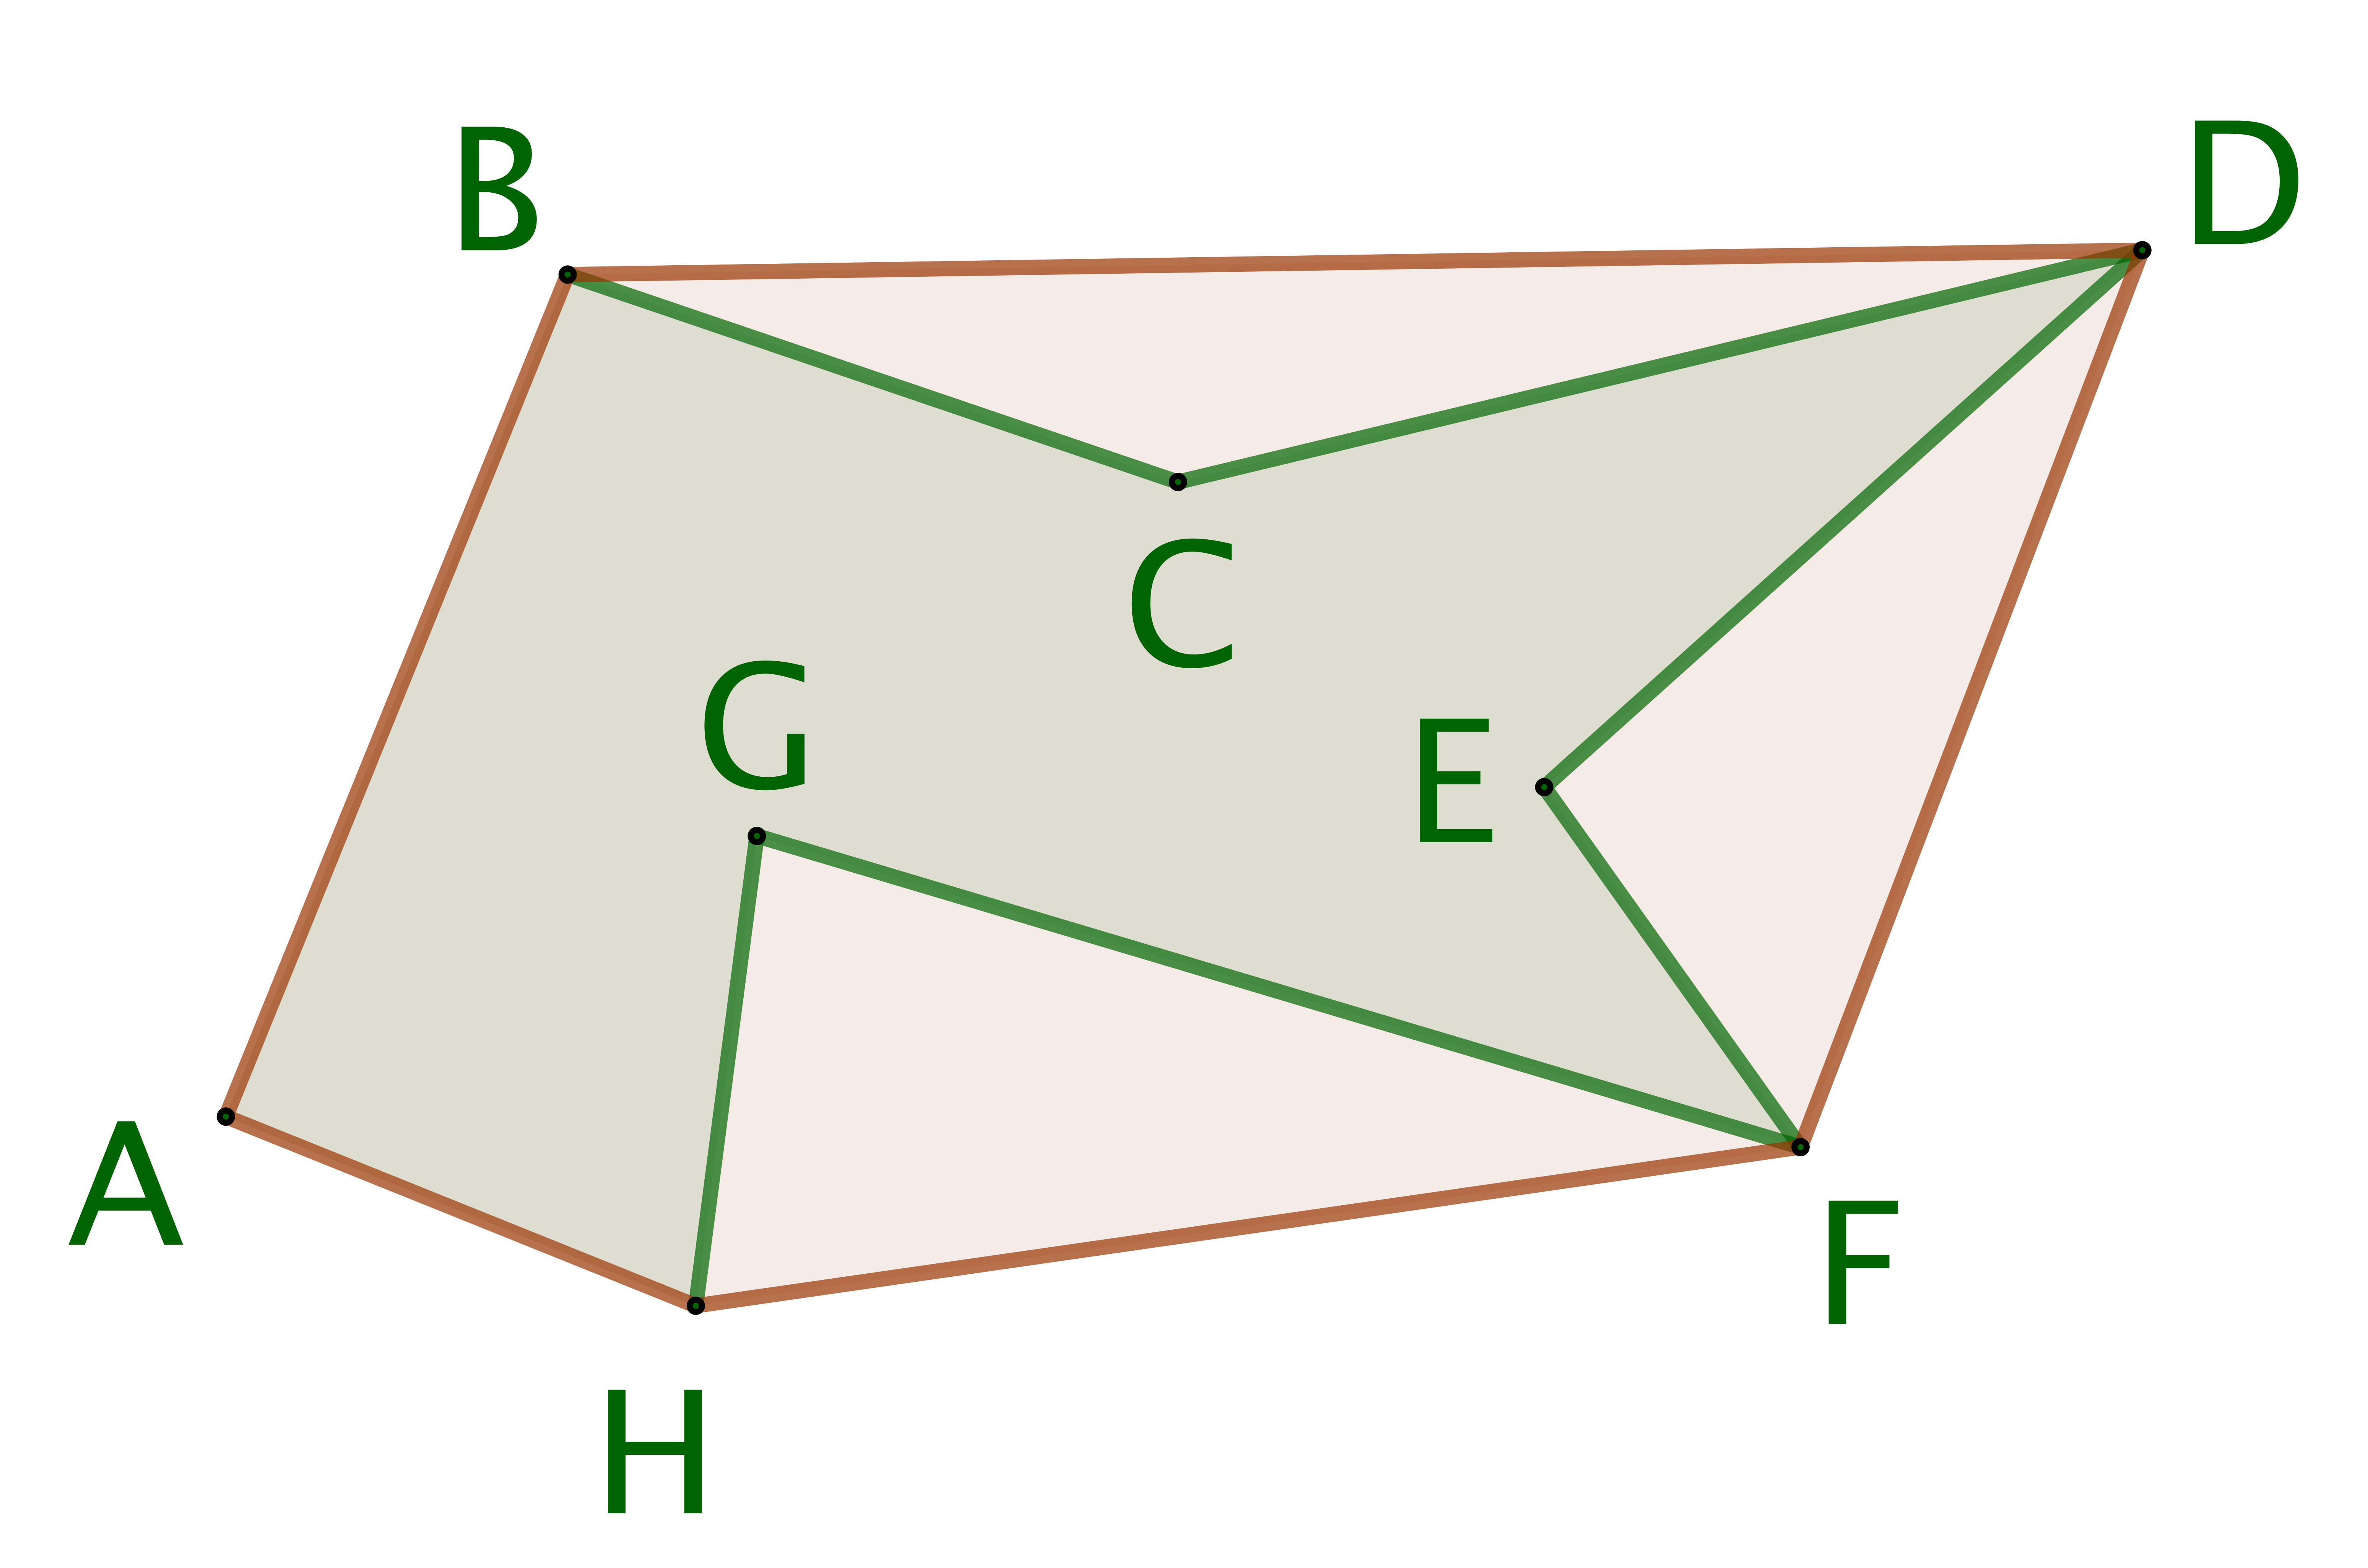
\includegraphics[scale=.2]{content/polygon/sol-must-be/convex-hull.png}
	\end{center}
	
	Clairement,
	$\perim{\setproba{E}} < \perim{\setproba{P}}$
	et
	$\area{\setproba{E}} > \area{\setproba{P}}$,
	mais
	$\setproba{E}$ est un \kgone\ avec $k < n$. 
	%
	Appliquons donc le fait \ref{bigger-convex} à $\setproba{E}$, $s = n - k$ et $L = \perim{\setproba{P}}$.
	Ceci nous donne un \ngone\ convexe $\primeit{\setproba{C}}$ vérifiant
	$ \area{\primeit{\setproba{C}}} > \area{\setproba{E}} > \area{\setproba{P}}$
	et
	$\perim{\setproba{E}} < \perim{\primeit{\setproba{C}}} < \perim{\setproba{P}}$.
	%
	Finalement, une homothétie de rapport $r > 1$, où $r = \frac{ \perim{\setproba{P}} }{ \perim{\primeit{\setproba{C}}} }$, donne le \ngone\ convexe $\setproba{C}$ cherché.
	
	\null\vspace{-5ex}
\end{proof}


% ----------------------- %


\begin{fact} \label{must-be-equi}
	Si un \ngone\ convexe $\setproba{P}$ n'est pas équilatéral,
	alors nous pouvons construire un \ngone\ convexe $\setproba{C}$ tel que
	$\perim{\setproba{C}} = \perim{\setproba{P}}$
	et
	$\area{\setproba{C}} > \area{\setproba{P}}$.
\end{fact}


\begin{proof}
	Considérons un \ngone\ convexe non équilatéral $\setproba{P}$,
	de sorte que $\setproba{P}$ admet un triplet de sommets consécutifs $A$, $B$ et $C$ tels que $AB \neq BC$
	(sinon, on obtiendrait, de proche en proche, l'équilatéralité).
	%
	La construction vue dans la preuve du fait \ref{tri-one-side-fixed} nous donne la solution: voir les dessins ci-après où 
	$m$ est la médiatrice du segment $[AC]$,
	et
	$(AC) \parallel (BB^{\,\prime})$..
	%
	\begin{multicols}{2}
		\centering

		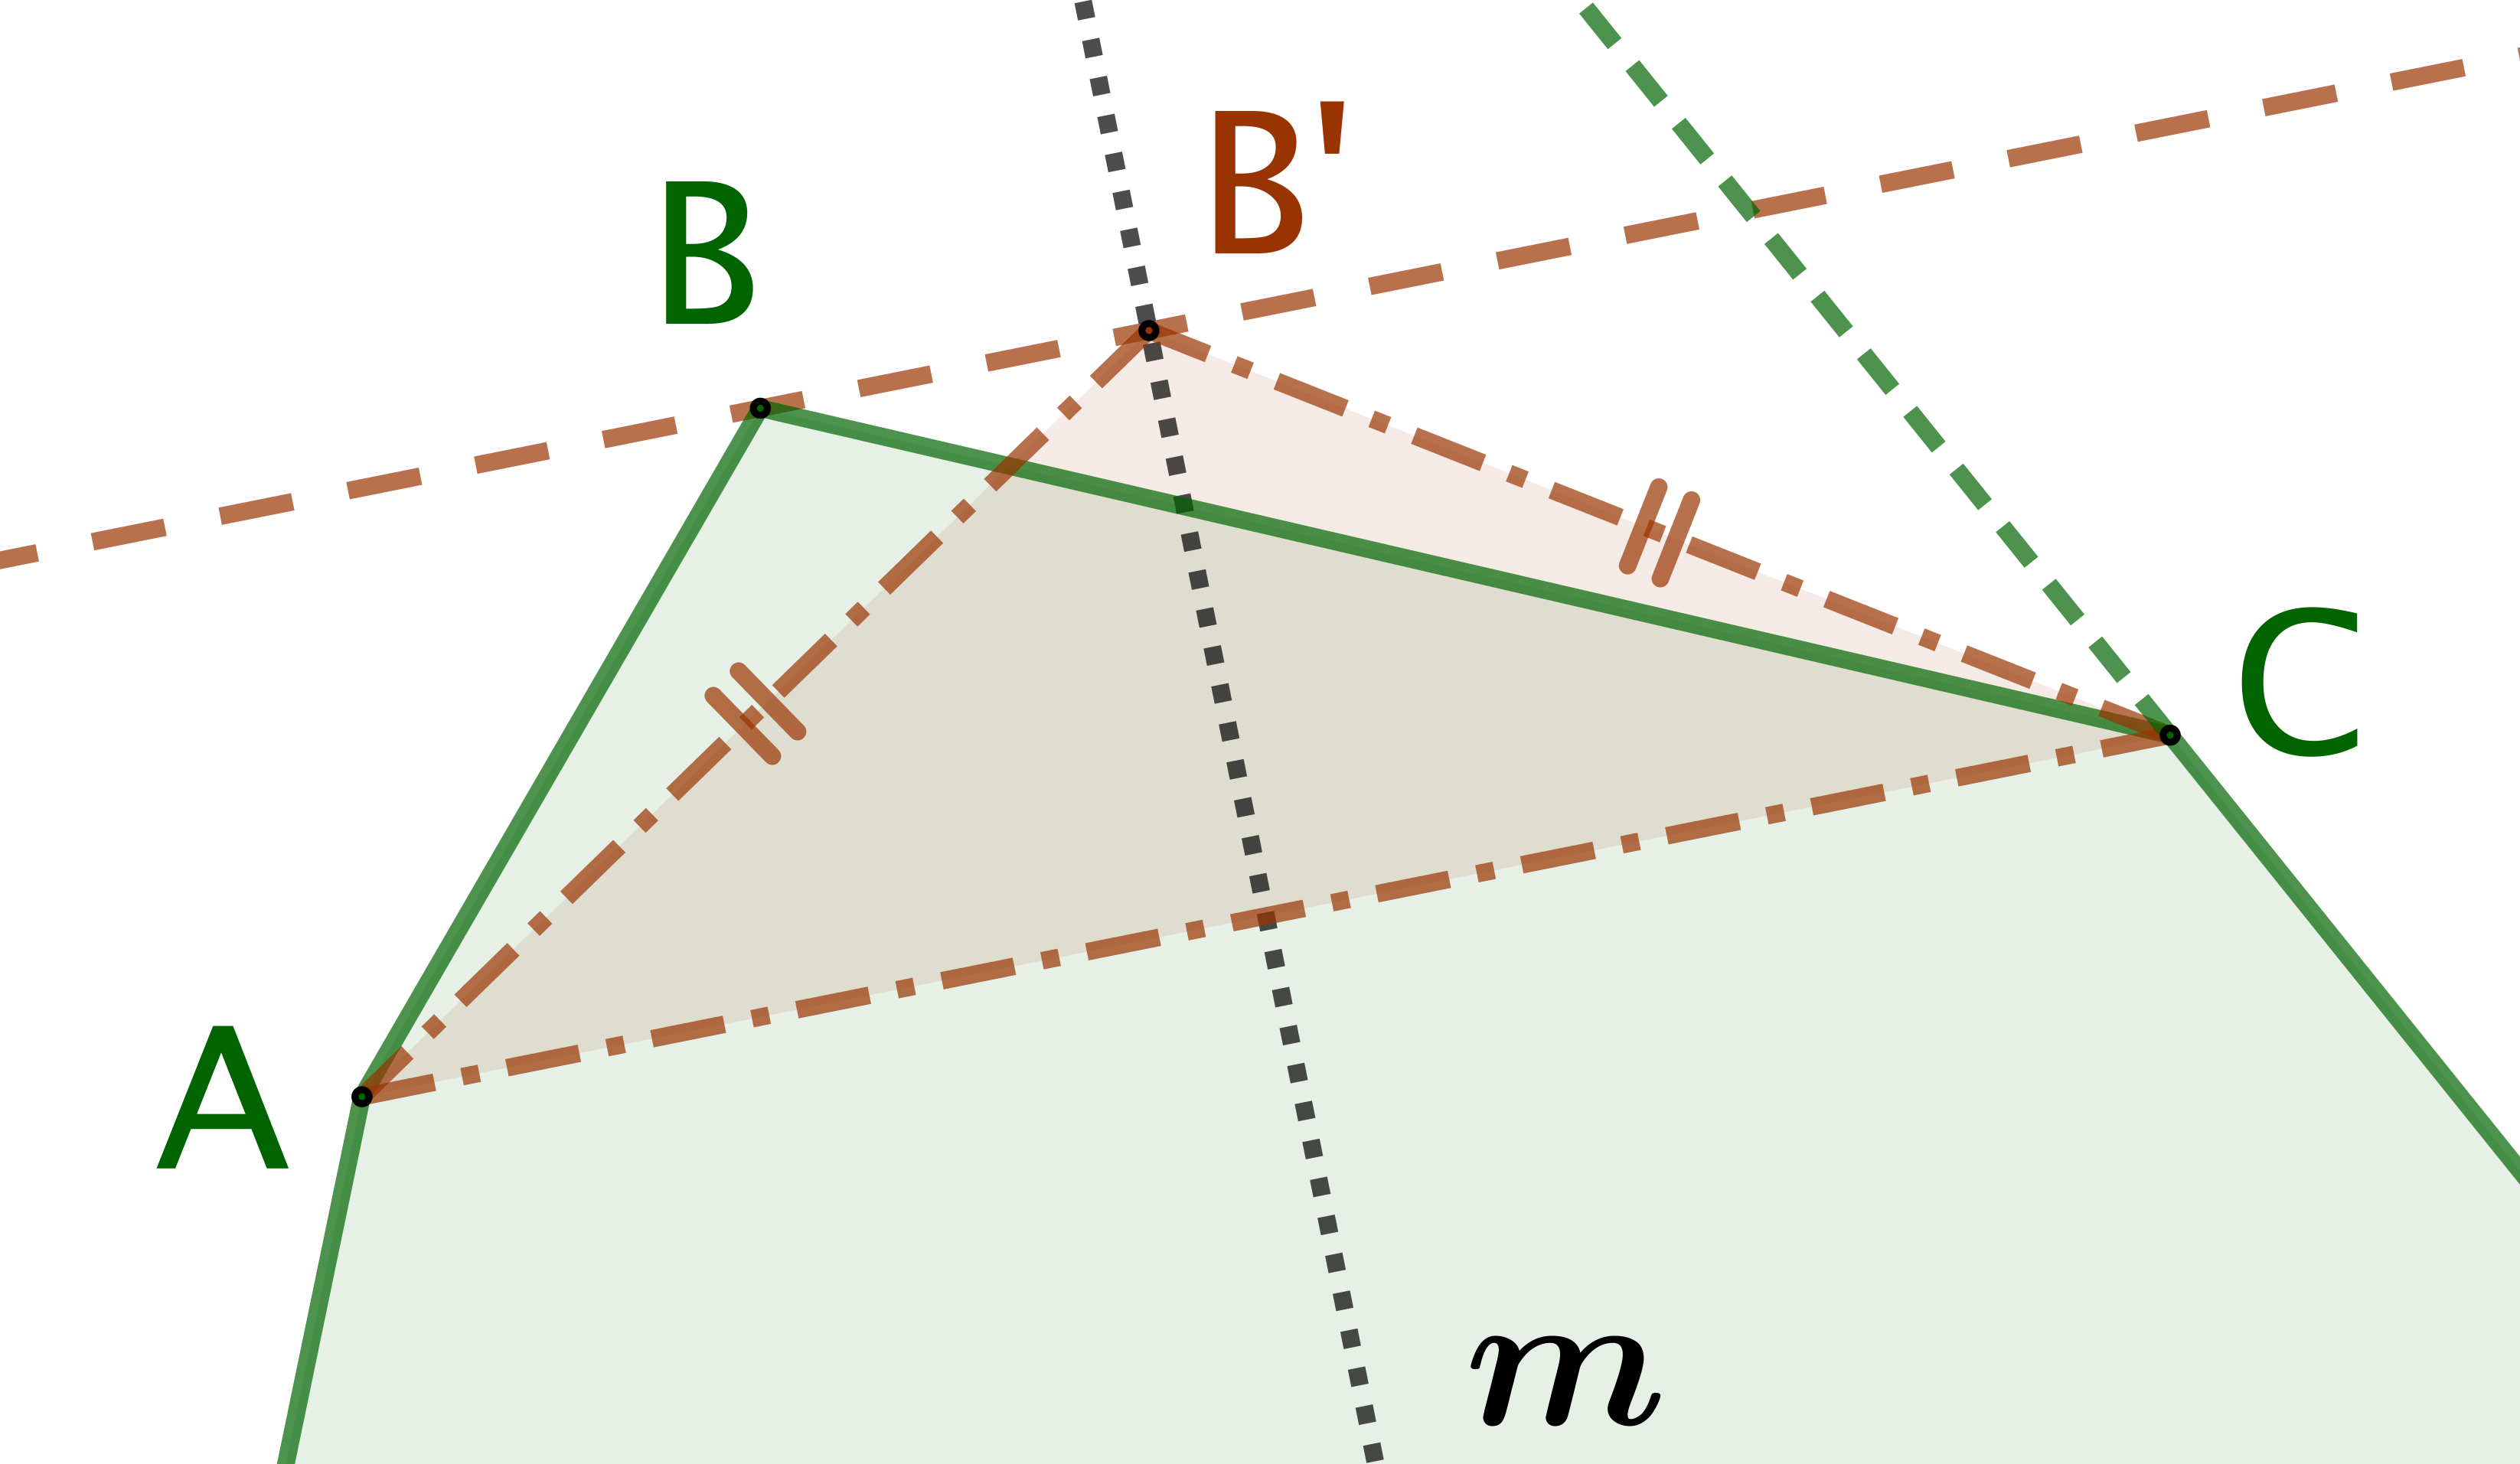
\includegraphics[scale=.35]{content/polygon/sol-must-be/not-iso-IN.png}

		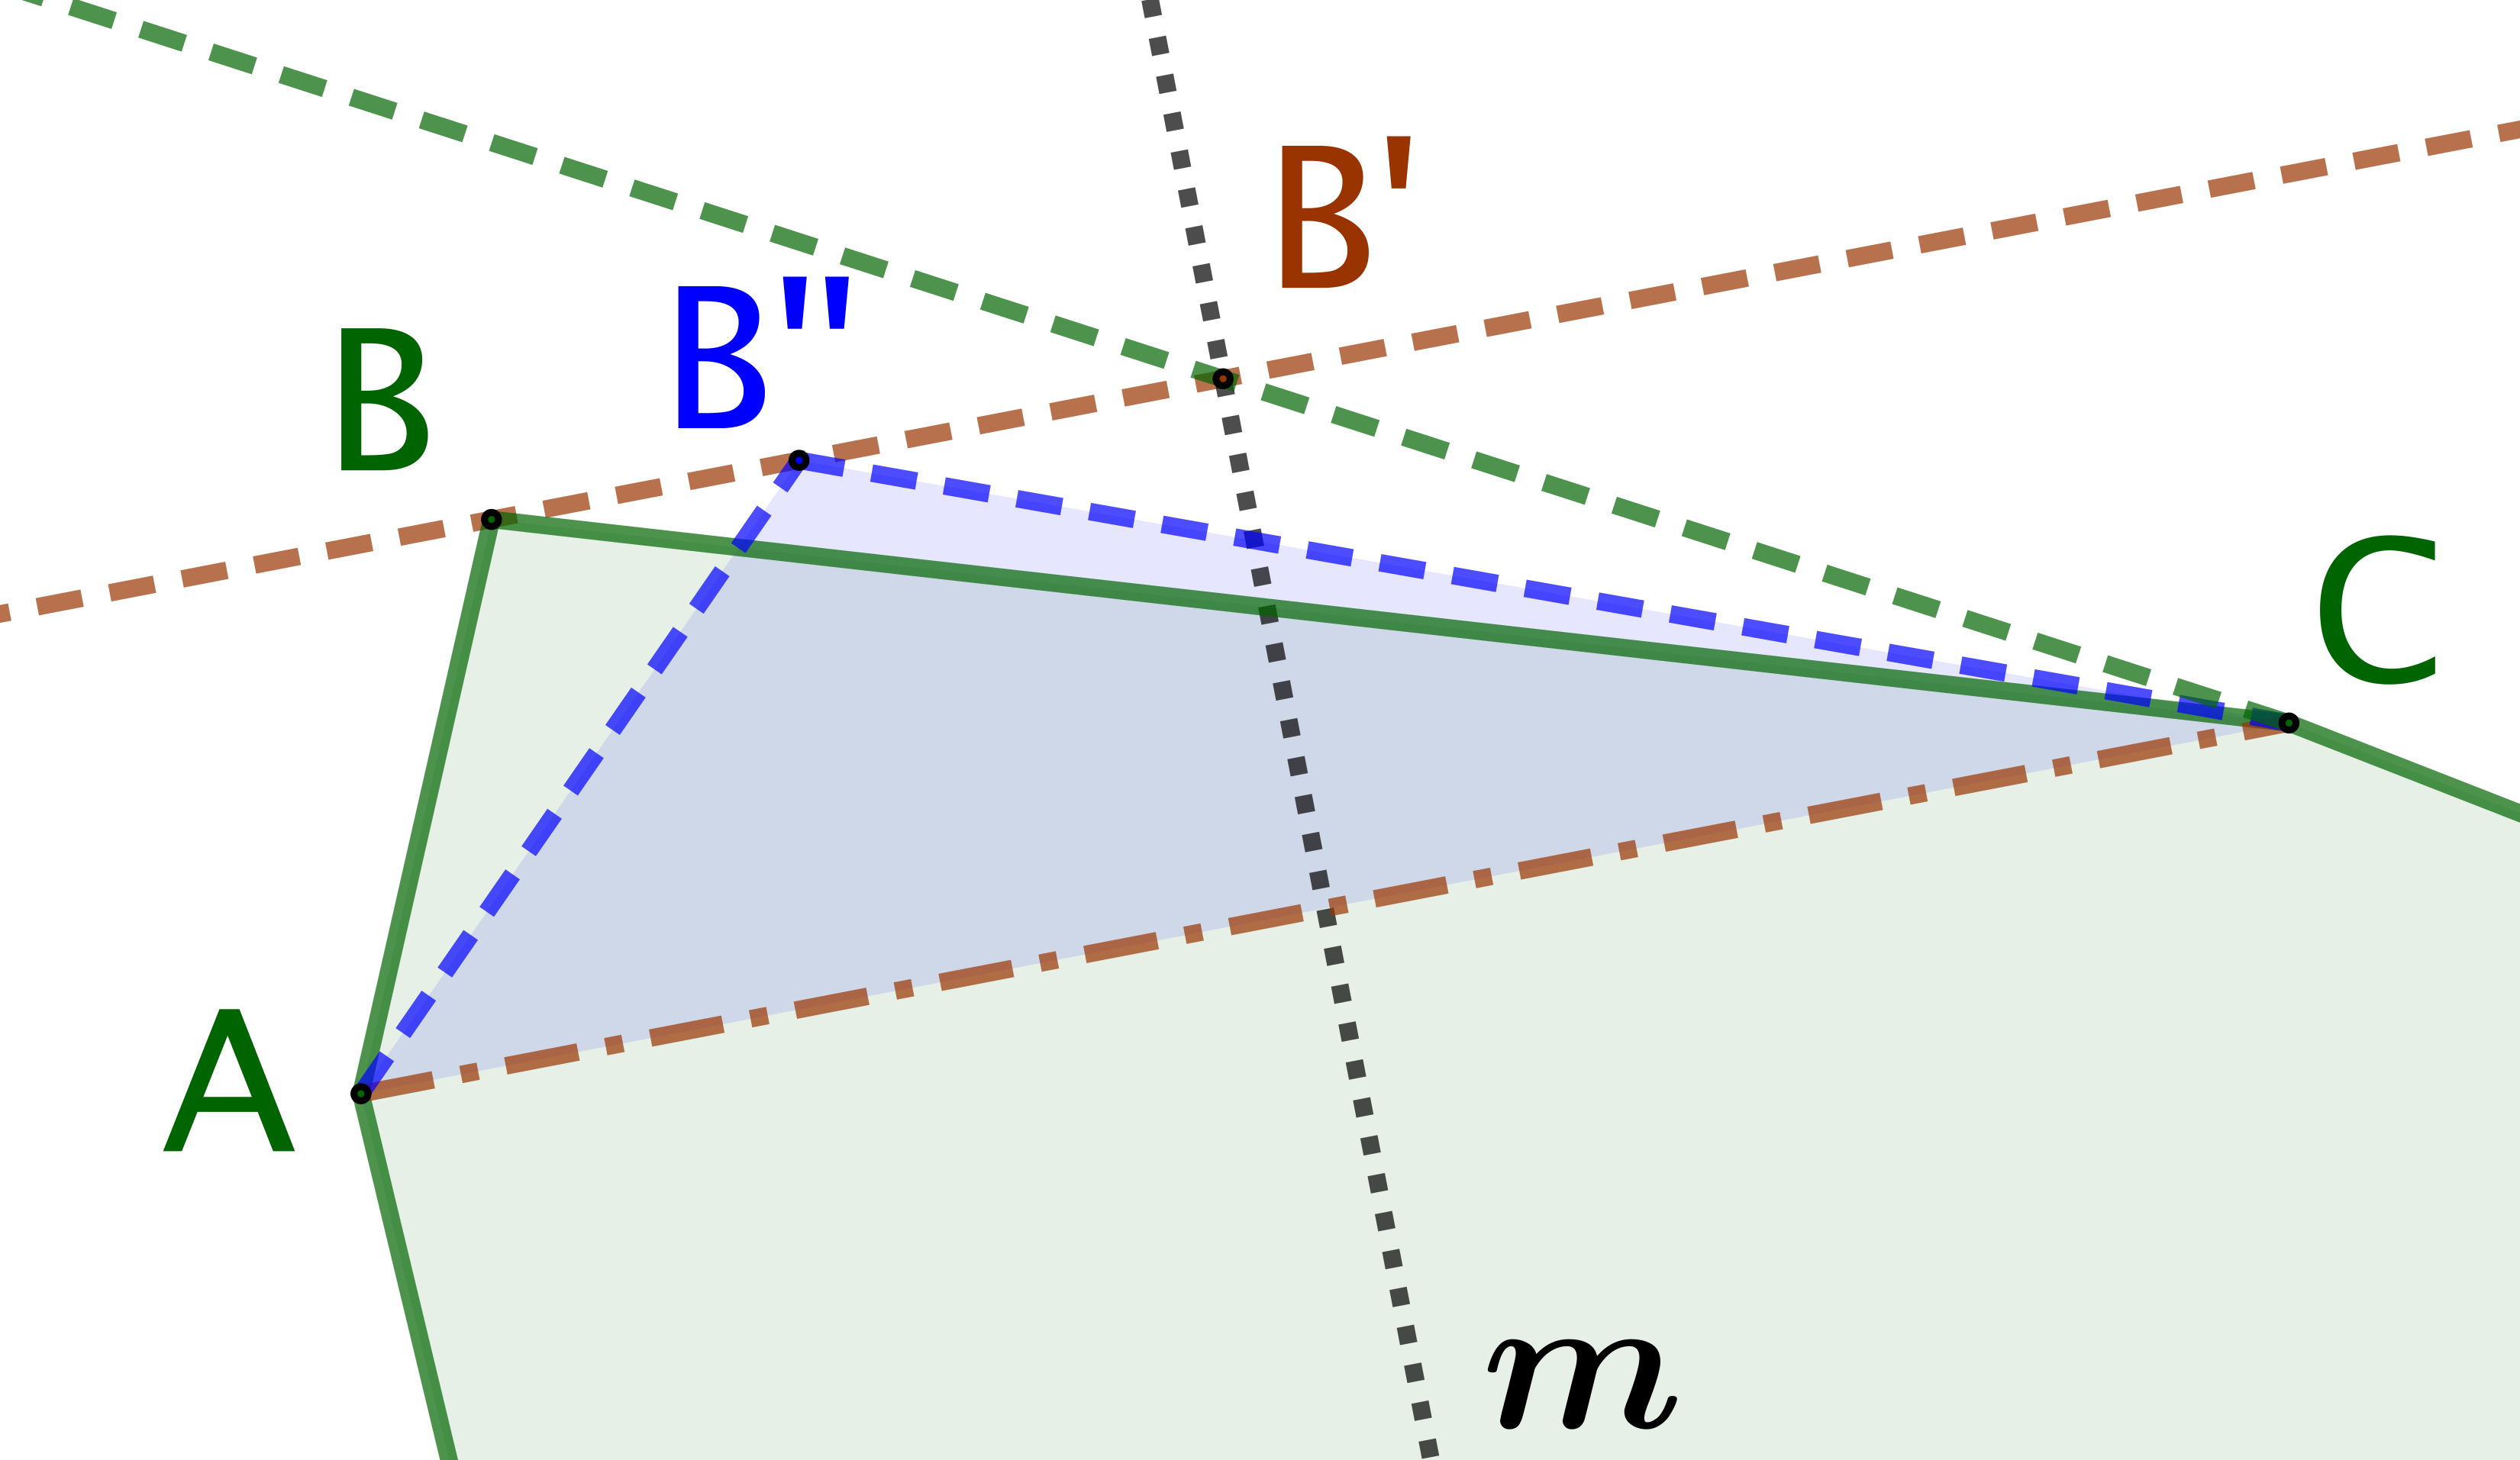
\includegraphics[scale=.35]{content/polygon/sol-must-be/not-iso-BORDER.png}
	\end{multicols}


	Il faut bien noter que pour le 2\ieme\ cas ci-dessus, il n'est pas possible d'utiliser le triangle $AB^{\,\prime}C$ isocèle en $B^{\,\prime}$, sinon nous n'aurions plus un \ngone.
	Pour ces situations problématiques, il suffit de se \focus{déplacer} un peu sur le segment ouvert $]BB^{\,\prime}[$ en direction de $m$.
	%
	Quoiqu'il en soit, dans chaque cas, nous avons construit un \ngone\ convexe $\primeit{\setproba{C}}$ tel que
	$\perim{\primeit{\setproba{C}}} < \perim{\setproba{P}}$
	et
	$\area{\primeit{\setproba{C}}} = \area{\setproba{P}}$.
	Une homothétie de rapport $r > 1$, où $r = \frac{ \perim{\setproba{P}} }{ \perim{\primeit{\setproba{C}}} }$, donne le \ngone\ convexe $\setproba{C}$ cherché.
\end{proof}


\begin{remark}
	Le fait précédent ne permet pas de toujours se ramener au cas d'un \nequi\ convexe. Il nous dit juste que si un \ngone\ convexe maximise son aire à périmètre fixé, alors il devra être, a minima, un \nequi. La nuance est importante, et une similaire existe pour la conclusion du fait suivant.
\end{remark}


% ----------------------- %


\begin{fact} \label{must-be-iso}
	Si un \nequi\ convexe $\setproba{P}$ n'est pas équiangle,
	alors il existe un \ngone\ convexe $\setproba{C}$ tel que
	$\perim{\setproba{C}} = \perim{\setproba{P}}$
	et
	$\area{\setproba{C}} > \area{\setproba{P}}$.
\end{fact}


\begin{proof}
	Considérons un \nequi\ convexe non équiangle $\setproba{P}$, 
	de sorte que $\setproba{P}$ admet un quadruplet de sommets consécutifs $A$, $B$, $C$ et $D$ tels que $\anglein{ABC} \neq \anglein{BCD}$
	(sinon, on obtiendrait, de proche en proche, l'équiangularité).
	Quitte à changer l'ordre de parcours des sommets de $\setproba{P}$, nous pouvons supposer $\anglein{ABC} > \anglein{BCD}$.
	%
	\begin{center}
		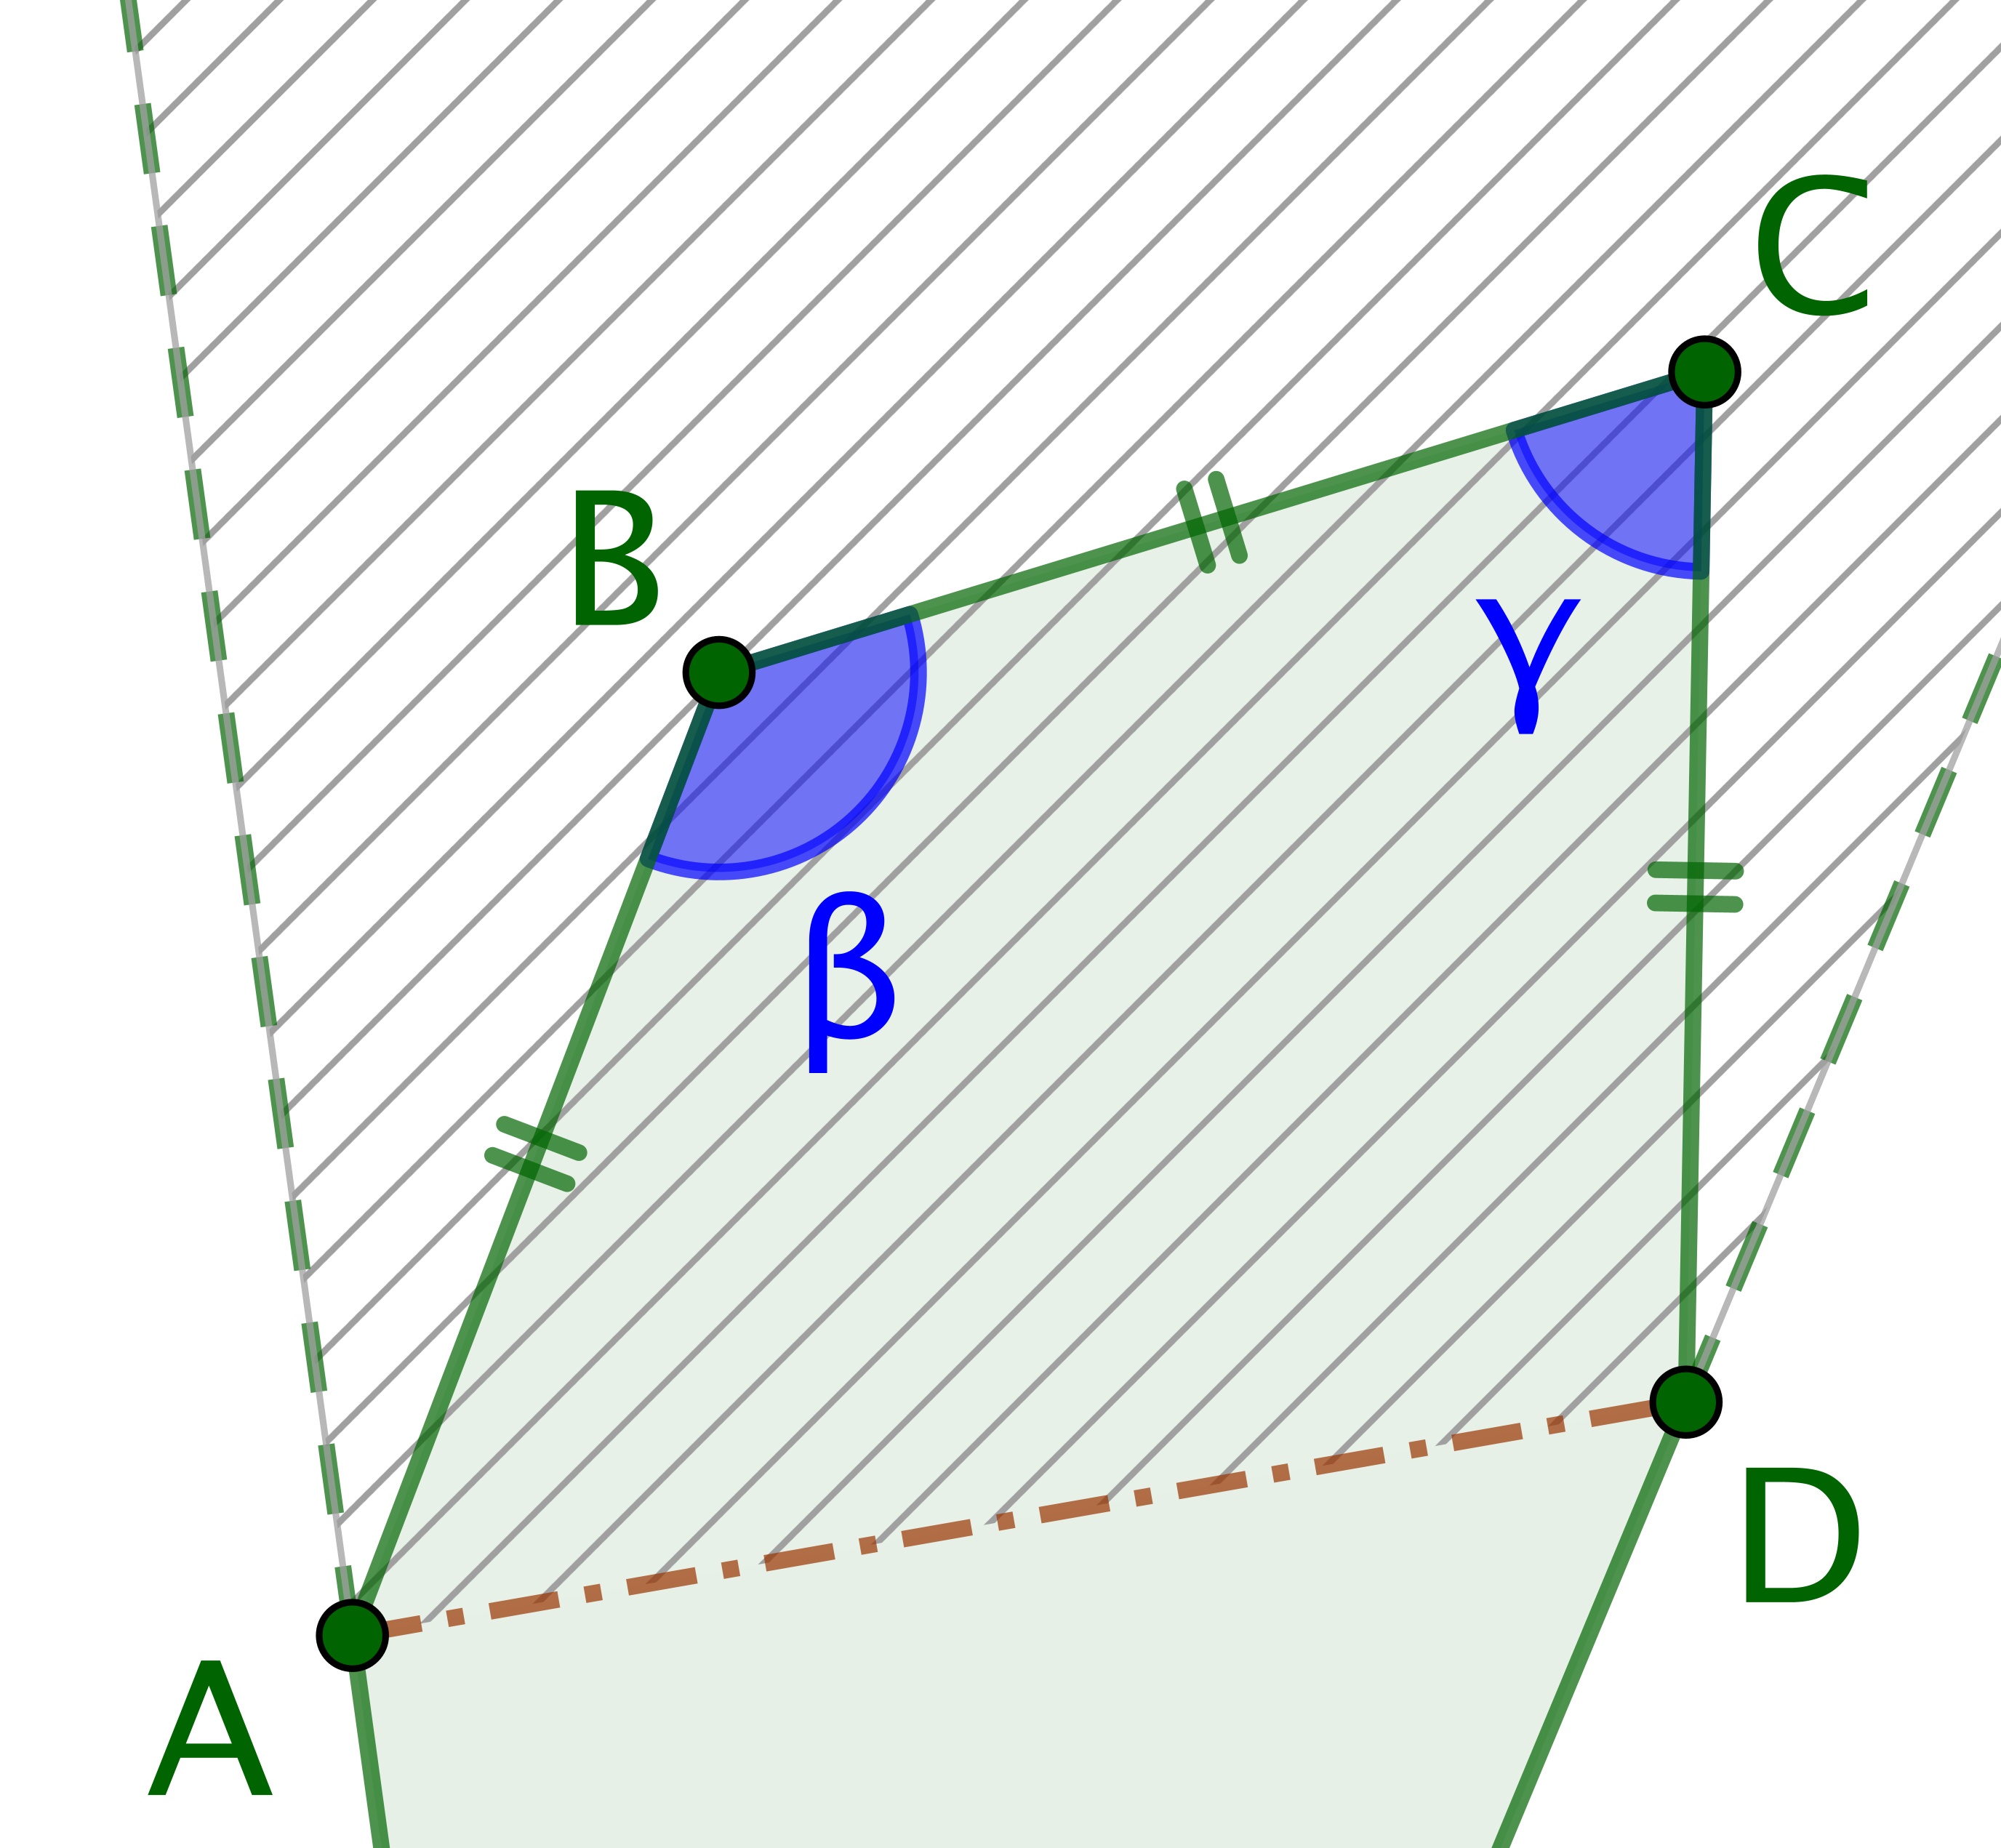
\includegraphics[scale=.4]{content/polygon/sol-must-be/2-eq-angles-start.png}
	\end{center}
	
	Nous garderons un \ngone\ convexe si nous déplaçons $B$ et $C$ dans la zone hachurée qui est à l'extérieur du \ngone, et strictement entre les droites en pointillés, portées par des côtés contigus à $[AB]$ et $[CD]$.
	%
	Concentrons-nous donc sur le quadrilatère $ABCD$, et posons $c = AB$ la longueur commune des côtés de $\setproba{P}$, ainsi que $d = AD$, une longueur que nous ne pouvons pas modifier, car $A$ et $D$ doivent rester fixés.
	%
	Nous pouvons construire $C$ comme suit via des cercles de rayon $c$ centrés en $A$ et $D$ fixes, et en $B$ mobile.
	%
	\begin{center}
		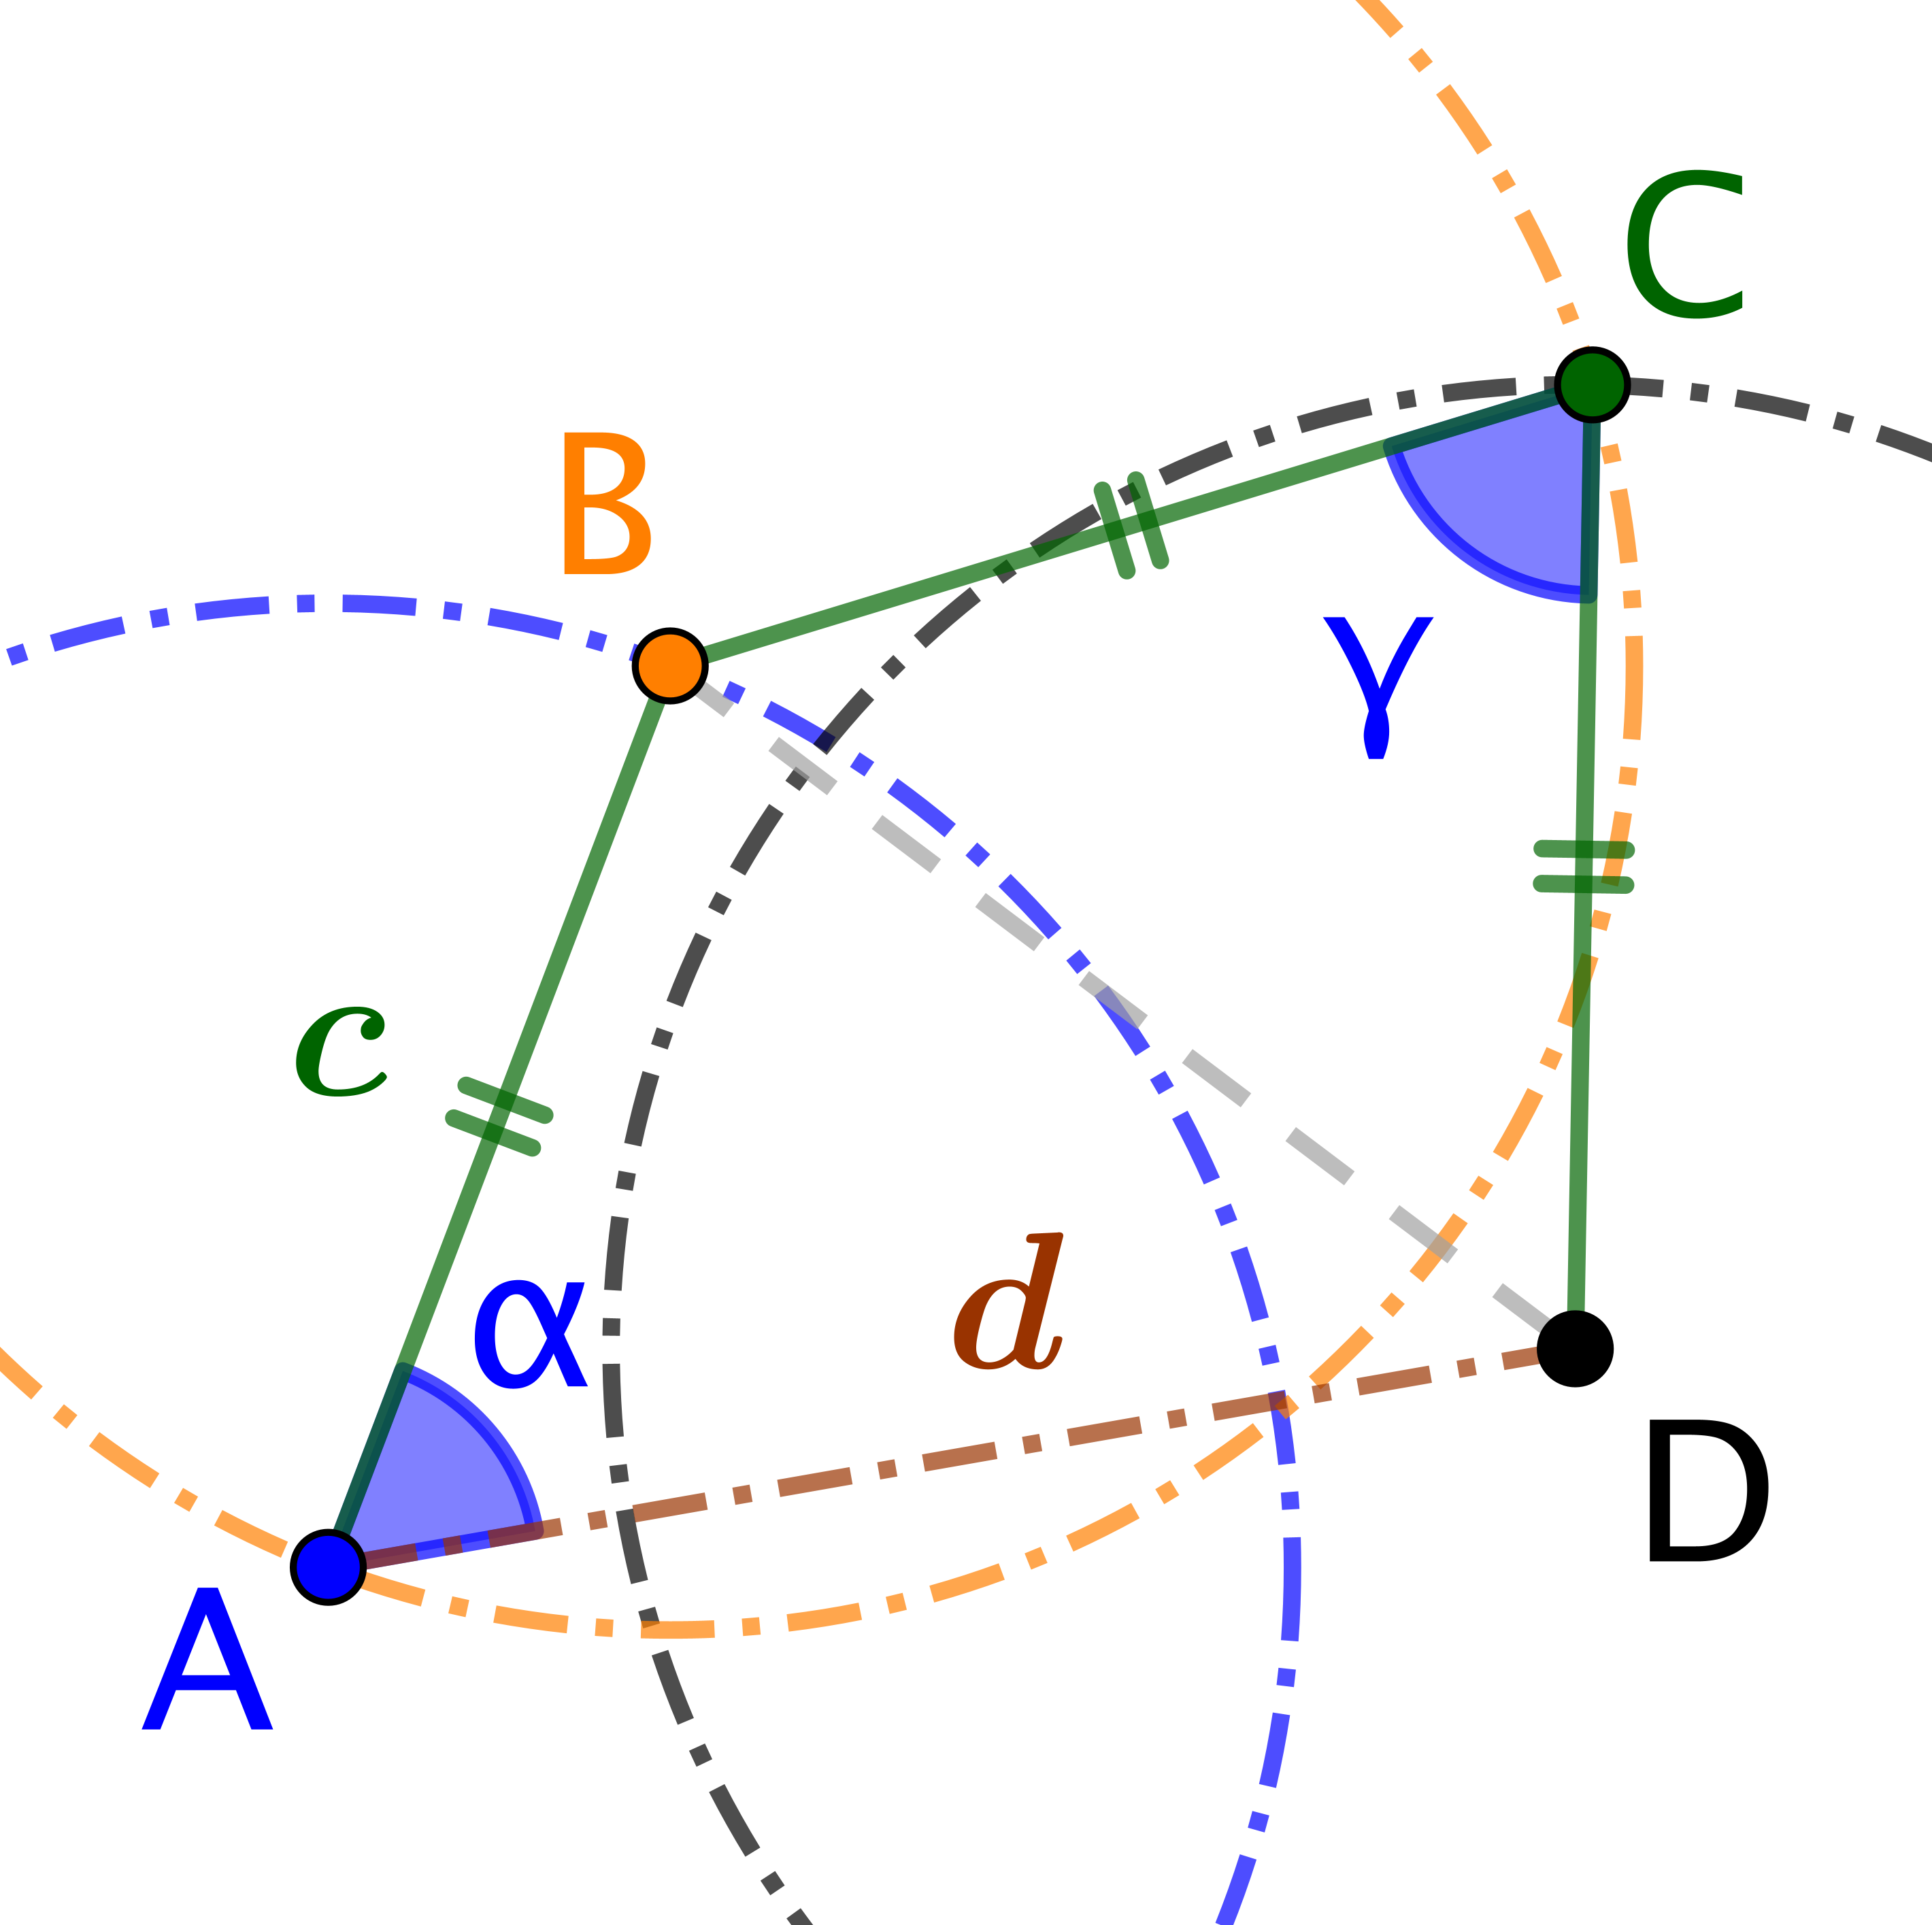
\includegraphics[scale=.35]{content/polygon/sol-must-be/2-eq-angles-circle.png}
	\end{center}

	Cherchons alors à exprimer $\area{ABCD}$ en fonction de $\alpha = \anglein{DAB}$, cet angle permettant de repérer le point mobile $B$.
	%
	\begin{itemize}
	    \item Par convexité, nous avons $\alpha \in \intervalO{0}{\pi}$ et $\gamma \in \intervalO{0}{\pi}$.


	    \item Le théorème d'Al-Kashi donne
	    $BD^2 = c^2 + d^2 - 2 c d \cos \alpha$ dans le triangle $ABD$,
	    ainsi que
	    $BD^2 = 2 c^2 - 2 c^2 \cos \gamma$ dans le triangle $BCD$.
	    Donc,
	    $2 \cos \gamma = 1 - k^2 + 2 k \cos \alpha$ où l'on a posé $k = \frac{d}{c}$.
	    Notons que l'inégalité triangulaire donne $d < 3 c$, puis $0 < k < 3$.


	    \item La formule trigonométrique de l'aire d'un triangle donne
	    $\area{ABD} = \num{.5} c d \sin \alpha$
	    et
	    $\area{BCD} = \num{.5} c^2 \sin \gamma$,
	   	puis
	    $\area{ABCD} = \num{.5} c^2 ( k \sin \alpha + \sin \gamma )$,
	    de sorte que
    	$\area{ABCD} = \num{.5} c^2 f(\alpha)$
    	en posant 
    	$f(\alpha) = k \sin \alpha + \sqrt{1 - \num{.25} ( 1 - k^2 + 2 k \cos \alpha)^2}$,
	    car 
	    $\sin \gamma = \sqrt{1 - \cos^2 \gamma}$.


	    \item Passons à l'étude de $\sder{f}{1}(\alpha) = 0$, en nous souvenant que nous n'avons pas besoin d'atteindre le maximum de $f$, mais juste de pouvoir faire augmenter localement $f(\alpha)$. 
	    Dans les implications suivantes, nous avons posé 
	    $\onelist{S} = \sin \alpha$ et $\onelist{C} = \cos \alpha$.
	    
	    \leavevmode\kern-2em%
	    \begin{stepcalc}[style=ar*, ope={\implies[d'où]}]
	        \sder{f}{1}(\alpha) = 0
	    \explnext{}
	        k \onelist{C}
	        +
	        \frac{ k \onelist{S} ( 1 - k^2 + 2 k \onelist{C}) }{ 2 \sqrt{1 -  \num{.25} ( 1 - k^2 + 2 k \onelist{C})^2} }
	        =
	        0
	    \explnext{}
	        \onelist{S} ( 1 - k^2 + 2 k \onelist{C}) 
	        =
	        - 2 \onelist{C} \sqrt{1 - \num{.25} ( 1 - k^2 + 2 k \onelist{C})^2}
	    \explnext{}
	        \onelist{S}^2 ( 1 - k^2 + 2 k \onelist{C})^2
	        =
	        4 \onelist{C}^2 \big( 1 - \num{.25} ( 1 - k^2 + 2 k \onelist{C})^2 \big)
	    \explnext{}
	        ( 1 - k^2 + 2 k \onelist{C})^2 (\onelist{S}^2 + \onelist{C}^2)
	        =
	        4 \onelist{C}^2
	    \explnext*{$\onelist{C}^2 + \onelist{S}^2 = 1$}{}
	        ( 1 - k^2 + 2 k \onelist{C})^2 - 4 \onelist{C}^2 = 0
	    \end{stepcalc}
	    
	    \noindent
	    Les implications se poursuivent comme suit.
	    
	    \leavevmode\kern-2em%
	    \begin{stepcalc}[style=ar*, ope={\implies[d'où]}]
	        ( 1 - k^2 + 2 k \onelist{C})^2 - 4 \onelist{C}^2 = 0
	    \explnext{}
	        ( 1 - k^2 + 2 k \onelist{C} - 2 \onelist{C} )
	        \,
	        ( 1 - k^2 + 2 k \onelist{C} + 2 \onelist{C} )
	        = 0
	    \explnext{}
	        (1 - k) ( 1 + k - 2 \onelist{C} )
	        \,
	        (1 + k) ( 1 - k + 2 \onelist{C} ) = 0
	    \explnext*{$k > 0$}{}
	        k = 1
	        \,\, \text{ou} \,\,
	        \onelist{C} \in \setgene{ \frac{k - 1}{2} , \frac{k + 1}{2} }
	    \end{stepcalc}


	    \item $k = 1$ signifie que $ABCD$ est un losange, non rectangle, car $\anglein{ABC} \neq \anglein{BCD}$.
	    Dans ce cas, en bougeant un peu le sommet $B$ parallèlement à $(AD)$, tout en faisant
	    augmenter $\alpha$ légèrement si $\alpha \in \intervalO{0}{\frac{\pi}{2}}$,
	    ou
	    diminuer $\alpha$ légèrement si $\alpha \in \intervalO{\frac{\pi}{2}}{\pi}$,%
	    \footnote{
	        $B$ se déplace vers la gauche dans notre cas.
	    }
	    nous obtenons un parallélogramme de même aire, mais de périmètre diminué,%
	    \footnote{
	        Si besoin, se reporter à la preuve du fait \ref{iso-para}.
	    }
	    et par conséquent un \ngone\ convexe $\primeit{\setproba{C}}$ tel que
		$\perim{\primeit{\setproba{C}}} < \perim{\setproba{P}}$
		et
		$\area{\primeit{\setproba{C}}} = \area{\setproba{P}}$,
		qu'il suffit d'agrandir homothétiquement pour conclure.


	    \item Pour $k \neq 1$ et $\onelist{C} = \frac{k - 1}{2}$,
	    nous avons $2\cos \alpha = k - 1$, 
	    puis 
	    $2 \cos \gamma = 1 - k^2 + k(k - 1) = 1 - k$,
	    soit
	    $\cos \gamma = - \cos \alpha$ qui fournit
	    $\gamma = \pi - \alpha$, en se souvenant que $(\alpha , \gamma) \in \intervalO{0}{\pi}^2$.
	    Notons que $\alpha \neq \frac{\pi}{2}$ et $\gamma \neq \frac{\pi}{2}$, car $k \neq 1$. 
	    Nous aboutissons à la contradiction que $ABCD$ est un trapèze isocèle de bases $[AD]$ et $[BC]$, ceci impliquant $\anglein{ABC} = \anglein{BCD}$. 
	    L'isocélité vient des points suivants.
	    %
	    \begin{enumerate}
	        \item Notre construction de $C$ à base de cercles est déterministe, car $B$ et $C$ sont situés dans le même demi-plan délimité par $(AD)$.

	        \item Si $\primeit{A} \primeit{B} \primeit{C} \primeit{D}$ est un trapèze isocèle de bases $[\primeit{A} \primeit{D}]$ et $[\primeit{B} \primeit{C}]$, via la somme des angles aux sommets d'un quadrilatère convexe, qui vaut $(4 - 2) \pi = 2 \pi$, nous avons
	        $\anglein{\primeit{B} \primeit{C} \primeit{D}} = \pi - \anglein{\primeit{D} \primeit{A} \primeit{B}}$.

	        \item Comme $2 \cos \gamma = 1 - k^2 + 2 k \cos \alpha$ pour $(\alpha, \gamma) \in \intervalO{0}{\pi}^2$,
	        nous avons:
	        $\gamma = \pi - \alpha$ si, et seulement si, $\cos \alpha = \frac{k - 1}{2}$.
	    \end{enumerate}


	    \item Pour $k \neq 1$ et $\onelist{C} = \frac{k + 1}{2}$,
	    comme au début du point précédent,
	    nous avons $\cos \gamma = \cos \alpha$, puis $\gamma = \alpha$ avec $(\alpha , \gamma) \in \intervalO{0}{\pi}^2$.
	    Notons qu'ici $0 < k < 1$, puis $(\alpha , \gamma) \in \intervalO{0}{\frac{\pi}{3}}^2$.
	    Dès lors, les monotonies de $\sin$ et $\cos$ sur $\intervalO{0}{\frac{\pi}{3}}$, combinées à $1 - k^2 + 2 k \cos \alpha \geq 0$, impliquent la stricte croissance de $f$ sur $\intervalO{0}{\frac{\pi}{3}}$.%
	    \footnote{
	    	Nous utilisons la composition de fonctions monotones, ce qui n'est pas toujours faisable.
	    }
	    Il suffit donc d'augmenter légèrement la valeur de  $\alpha$, ceci étant faisable d'après la construction à base de cercles.
	\end{itemize}
	
	\null\vspace{-6ex}
\end{proof}


\begin{remark}
    Ce qui précède donne envie de faire appel à la méthode des extrema liés pour plus d'élégance, et d'efficacité, dans les calculs, modulo l'utilisation d'un gros théorème.
    Étudions donc les extrema de
	$f(\alpha , \gamma) = k \sin \alpha + \sin \gamma$
	sur $\intervalO{0}{\pi}^2$, qui est un ouvert,
	sous la contrainte $g(\alpha , \gamma) = 0$
	avec
	$g(\alpha , \gamma) = 1 - k^2 + 2 k \cos \alpha - 2 \cos \gamma$.
	%
    Si un extremum existe, alors nous avons $\lambda \in \RR$ tel que
    $\pder[i]{f}{\alpha}{1} = \lambda \pder[i]{g}{\alpha}{1}$
	et
    $\pder[i]{f}{\gamma}{1} = \lambda \pder[i]{g}{\gamma}{1}$,
	de sorte que
	$k \cos \alpha = - 2 k \lambda \sin \alpha$,
	soit
	$\cos \alpha = - 2 \lambda \sin \alpha$,
	et nous avons aussi
	$\cos \gamma = 2 \lambda \sin \gamma$.
	Nous aboutissons alors aux deux alternatives suivantes qui rejoignent les arguments de la preuve précédente.
	%
	\begin{enumerate}
	    \item Si $\lambda = 0$,
	    alors
	    $\alpha = \gamma = \frac{\pi}{2}$ et $k = 1$. 

	    \item Si $\lambda \neq 0$,
	    alors
	    $\cos \alpha \sin \gamma = - \sin \alpha \cos \gamma$,
	    puis
	    $\sin (\alpha + \gamma) = 0$,
	    et
	    $\alpha + \gamma = \pi$.
	\end{enumerate}
\end{remark}


%\begin{remark}
%    OK ???
%    
%    À périmètre fixé, le trapèze isocèle de bases $[AD]$ et $[BC]$ est celui maximise l'aire parmi les quadrilatères $ABCD$ vérifiant $AB = BC = CD$.
%\end{remark}


\begin{remark}
	Une démonstration géométrique du fait \ref{must-be-iso} est possible via un résultat attribué à Zénodore%
	\footnote{
	    La preuve du résultat de Zénodore est un peu fastidieuse.
	}
	sur la maximisation de l'aire totale de deux triangles isocèles de bases fixées, et de périmètre total constant:
	ce résultat affirme que les deux triangles doivent avoir des angles en leur sommet principal de même mesure.
	Malheureusement, cette preuve peut \focus{échouer} lors de la disparition d'un sommet en choisissant la paire optimale de triangles isocèles pour construire un nouveau \ngone\ \focus{plus gros}.
\end{remark}


% ----------------------- %


\begin{fact} \label{must-be-reg}
    Si $\setproba{P}$ est un \ngone\ maximisant l'aire parmi les \ngones\ de périmètre fixé, alors $\setproba{P}$ ne peut être que régulier et convexe.
\end{fact}


\begin{proof}
    Si $\setproba{P}$ n'était pas régulier et convexe, alors 
    soit il ne serait pas convexe, 
    soit il serait convexe, mais pas équilatéral, 
    soit il serait convexe et équilatéral, mais pas équiangle.
    Or, aucune de ces alternatives n'est possible d'après les faits \ref{must-be-conv}, \ref{must-be-equi} et \ref{must-be-iso}.
\end{proof}


%% ----------------------- %
%   GARDER POUR LYCée !!!
%
%
%\begin{proof}
%    Rappelons que pour un \nreg\ convexe $\setproba{R}$,
%    $\perim{\setproba{R}} = 2 n \sin (\frac{\pi}{n}) \rho$
%    et
%	$\area{\setproba{R}} = n \sin (\frac{\pi}{n})  \cos (\frac{\pi}{n}) \rho^2$
%	où $\rho$ désigne le rayon du cercle circonscrit à $\setproba{R}$.
%	Ceci donne 
%	$\area{\setproba{R}} = \frac{\perim{\setproba{R}}^2}{4 n \tan (\frac{\pi}{n})}$,
%	puis amène à justifier que 
%	$k_1 \tan (\frac{\pi}{k_1}) > k_2 \tan (\frac{\pi}{k_2})$,
%	c'est-à-dire que la suite $\big( k \tan (\frac{\pi}{k}) \big)_{k \in \NN_{\geq 3}}$ est strictement décroissante.
%	Ce fait découle directement de la stricte décroissance de la fonction $f$ définie sur $\RR_{>2}$ par $f(x) = x \tan (\frac{\pi}{x})$,
%	celle-ci venant des équivalences logiques suivantes où $x > 2$, la dernière assertion étant vraie d'après la validité de $\sin X \leq X$ sur $\RRp$.
%
%	\begin{stepcalc}[style=ar*, ope={\iff[ssi]}]
%		\sder{f}{1}(x) < 0
%	\explnext{}
%		\tan (\frac{\pi}{x}) - \frac{\pi}{x \cos^2 (\frac{\pi}{x})} < 0
%	\explnext{}
%		\tan (\frac{\pi}{x}) < \frac{\pi}{x \cos^2 (\frac{\pi}{x})}
%	\explnext{$\frac{\pi}{x} \in \intervalO{0}{\frac{\pi}{2}}$}
%		\cos^2 (\frac{\pi}{x}) \tan (\frac{\pi}{x}) < \frac{\pi}{x}
%	\explnext{}
%		\cos (\frac{\pi}{x}) \sin (\frac{\pi}{x}) < \frac{\pi}{x}
%	\explnext{}
%		\frac{1}{2} \sin (\frac{2 \pi}{x}) < \frac{\pi}{x}
%	\explnext{}
%		\sin (\frac{2 \pi}{x}) < \frac{2 \pi}{x}
%	\end{stepcalc}
%	
%	\null\vspace{-3.5ex}
%\end{proof}
%
